
%%%%%%%%%%%%%%%%%%%%%%%%%%%%%%%%%%%%%%%%%%%%%%%%%%%%%%%%%%%%%%%%%%%%%%
% How to use writeLaTeX: 
%
% You edit the source code here on the left, and the preview on the
% right shows you the result within a few seconds.
%
% Bookmark this page and share the URL with your co-authors. They can
% edit at the same time!
%
% You can upload figures, bibliographies, custom classes and
% styles using the files menu.
%
%%%%%%%%%%%%%%%%%%%%%%%%%%%%%%%%%%%%%%%%%%%%%%%%%%%%%%%%%%%%%%%%%%%%%%

\documentclass[12pt]{article}

\usepackage{sbc-template}
\usepackage{amsmath}
\usepackage{color,soul}
\usepackage{graphicx,url}
\usepackage{multicol}
\usepackage{diagbox}
\usepackage[dvipsnames]{xcolor}
\usepackage{verbatim}
\usepackage{makecell}

\newcommand{\R}[1]{~\scriptsize{(#1)}}
\newtheorem{definition}{Definition}

%\usepackage[brazil]{babel}   
\usepackage[utf8]{inputenc}  

     
\sloppy

\title{SMSM: a Multidimensioanl Similarity Measure for Trajectory Stops and Moves}

\author{Andre L. Lehmann\inst{1}, Luis Otavio Alvares\inst{1}, Vania Bogorny\inst{1} }


\address{Programa de Pós-Graduação em Ciência da Computação \\Departamento de Informatica e Estatistica, Universidade Federal de Santa Catarina\\ Florianopolis, Santa Catarina, Brasil
  \email{andre.lehmann@posgrad.ufsc.br,alvares@inf.ufsc.br ,vania.bogorny@ufsc.br}
}

\begin{document} 

\maketitle

\begin{abstract}
For many years trajectory similarity research has focused on raw trajectories, considering only space and time information. With the trajectory semantic enrichment emerged the need for similarity measures that support space, time, and semantics. Although some trajectory similarity measure deal with all three dimensions, they consider only stops or raw trajectories, ignoring the moves. We claim that, for some applications, the movement between stops is as important as the stops, and they must be considered in the similarity analysis.
  In this article we propose SMSM, a novel similarity measure for semantic trajectories that considers both stops and moves.
  SMSM is evaluated with real trajectory data of CRAWDAD and Geolife. The results show that SMSM overcomes state-of-art measures.
\end{abstract}

\section{Introduction}

Trajectory similarity measuring has received significant attention in the last few years, and several different measures have been proposed, ranging from single raw trajectories to multidimensional semantic trajectories. Earlier works as \cite{vlachos2002discovering} and \cite{Chen:2005:RFS:1066157.1066213} are limited to the spatial properties of raw trajectories, basically considering trajectories as two-dimensional objects with only space and time information. A \emph{raw trajectory} is generally represented as a sequence of points $T=<p_1, p_2, ...p_n>$, with $p_i=(x_i,y_i,t_i)$ where $x,y$ is the position of the object in space at time instant $t$. An example of raw trajectory is shown in Figure \ref{fig:single_trajectory}. Some similarity measures for raw trajectories are LCSS (Longest Common SubSequence) \cite{vlachos2002discovering}, EDR (Edit Distance on Real sequences) \cite{Chen:2005:RFS:1066157.1066213}, NWED (Normalized Weighted Edit Distance) \cite{dodge2012} and UMS (Uncertain Movement Similarity) \cite{Furtado-UMS-2018}.

\begin{figure}[h]
\centering
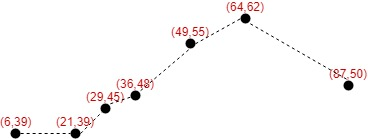
\includegraphics[width=0.5\textwidth]{Related_Works/Single_trajectory.jpg}
\caption{\label{fig:single_trajectory}An example of a raw trajectory}
\end{figure}


With the explosion of social media data and the need to represent movement over a more meaningful way, in 2008 emerged the concept of semantic trajectories\cite{Spaccapietra:2008:CVT:1347466.1347785}. Generally speaking, semantic trajectories are represented as \emph{sequences of stops and moves}, where \emph{stops} are the most important parts of trajectories, representing the places that an object has visited for a minimal amount of time, and the \emph{moves} are the trajectory points between stops. In several works, stops are called points of interest (POIs), episodes, or stay points. Semantic trajectories have at least three dimensions: space, time, and semantics. Figure \ref{fig:single_semantic_trajectory} shows an example of semantic trajectory.

\begin{figure}[h]
\centering
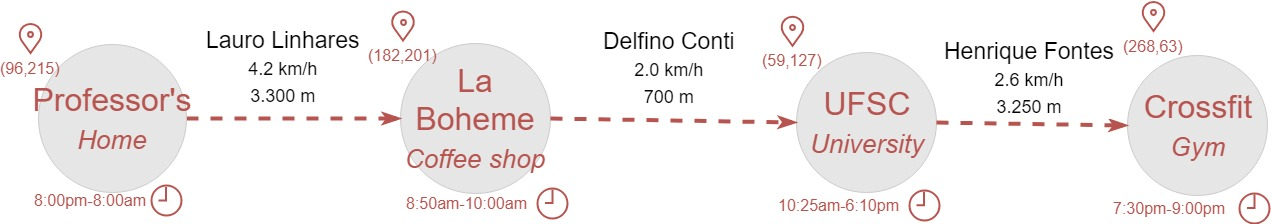
\includegraphics[width=0.9\textwidth]{Related_Works/Single_Semantic_trajectorie.jpg}
\caption{\label{fig:single_semantic_trajectory}An example of a semantic trajectory}
\end{figure}

\hl{In some applications, the {\emph{stops}} and {\emph{moves}} are more meaningful than a {\emph{raw}} trajectory. As example, we can use a sale promoter company. To company is more important the time (as short as possible) that a sale promoter is moving between stores than what was the travelled streets or what was the travelled distance. In this scenarios is clear that the semantic annotation of the \emph{moves} (the travelled time) is more relevant than the {\emph{raw}} trajectory points.

Figure {\ref{fig:involves_single_semantic_trajectory}} presents a sample trajectory of a sale promoter. The first {\emph{stop}} of trajectory is labeled as $A$, goes to $B$ and $C$ and ends in $D$. The {\emph{moves}} are the red points between {\emph{stops}}. As can be seen in Figure {\ref{fig:involves_single_semantic_trajectory}}, not whole trajectory has it points collected. Figure {\ref{fig:involves_similar_semantic_trajectory}} shows another trajectory from same user, visiting same stores, in the same order. As can be seen, the movement of both trajectories use the same street, but it GPS coordinates are in different locations, collected in a distinct rate. So, if a {\emph{raw}} trajectory similarity measure were used to compare both trajectories, this difference between the {\emph{move's}} points would decrease it similarity, even that the user had used same streets to move between stores.}

\begin{figure}[h]
\centering
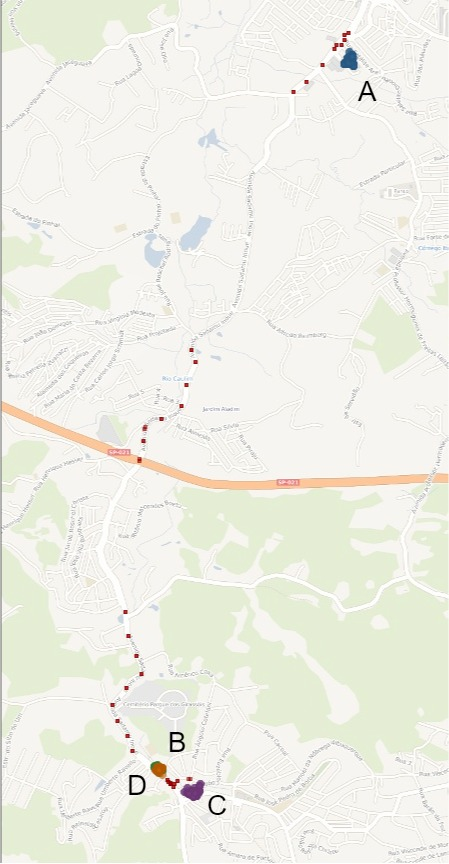
\includegraphics[width=0.3\textwidth]{Images/Involves-Trajectory.jpg}
\caption{\label{fig:involves_single_semantic_trajectory}A \emph{stop} and \emph{move} example trajectory of a sale promoter. The regions A, B, C and D are stores sale promoter works.}
\end{figure}

\begin{figure}[h]
\centering
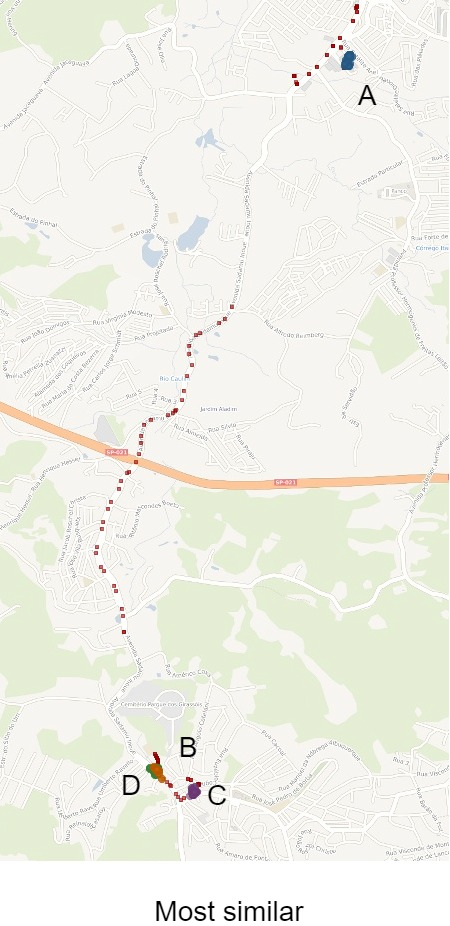
\includegraphics[width=0.3\textwidth]{Images/Involves-MostSimilarTrajectory.jpg}
\caption{\label{fig:involves_similar_semantic_trajectory}Another trajectory, with some movement points missing.}
\end{figure}

Although some similarity measures were proposed for semantic trajectories, they all suffer from the same problems: (i) do not address all three dimensions, as the works of \cite{Kang:2009:SMT:1529282.1529580} and \cite{Liu:2012:SMM:2442968.2442971}; (ii) address the similarity problem from a different perspective, considering the frequency of visited places, as the work of \cite{Ying:2010:MUS:1867699.1867703}; or (iii) exclusively address the \emph{stops}, systematically ignoring all information about the \emph{moves}, as the work of \cite{Furtado:TGIS12156}.

Similarity measures for semantic trajectories have not considered both stops and moves and the multidimensionality that characterizes semantic trajectories. The measure MSM, proposed by Furtado \cite{Furtado:TGIS12156}, for instance, considers only the stops, and they are treated as elements that are independent from each other, without considering the order as they appear in the trajectories. On the other hand, LCSS\cite{vlachos2002discovering} and EDR\cite{Chen:2005:RFS:1066157.1066213} consider the sequence of elements, but they force a match in all dimensions, not allowing partial similarity between trajectory elements. MD-DTW \cite{ten2007multi} is another approach that is able to handle multiple dimensions. It extends DTW \cite{berndt1994using} in order to find the distance between two sequences by looking for the best contiguous match of elements according to the sum of the distances in all dimensions. The problem of DTW and MD-DTW is that they consider the real distance between the elements, becoming sensitive to noise.

We claim that for several applications, the \emph{moves} are as important as the \emph{stops}, or even more important. \emph{Moves} carry important information such as the traveled distance from one place to another, the transportation means, the name of the streets over which the object has moved, the average speed, etc. \emph{Moves} are important for answering semantic queries such as (i) which objects go from place A to place B through the same roads? Which is the most popular route from A to B? Which is the average travel speed of trajectories moving from A to B following paths S1, S2, and S3 during rush hours? Figure \ref{fig:related_semantic_trajectories} shows an example of two semantic trajectories, where $P$ is the trajectory of a professor and $Q$ is the trajectory of the student. Notice that the trajectory \emph{stops} and \emph{moves} are composed of several data dimensions, considering space, time, and semantics. These data dimensions, that are of different data types, make the similarity problem more complex. The question we want to answer in this thesis is how similar are $P$ and $Q$ given both \emph{stops} and \emph{moves}?

\begin{figure}[!h]
\centering
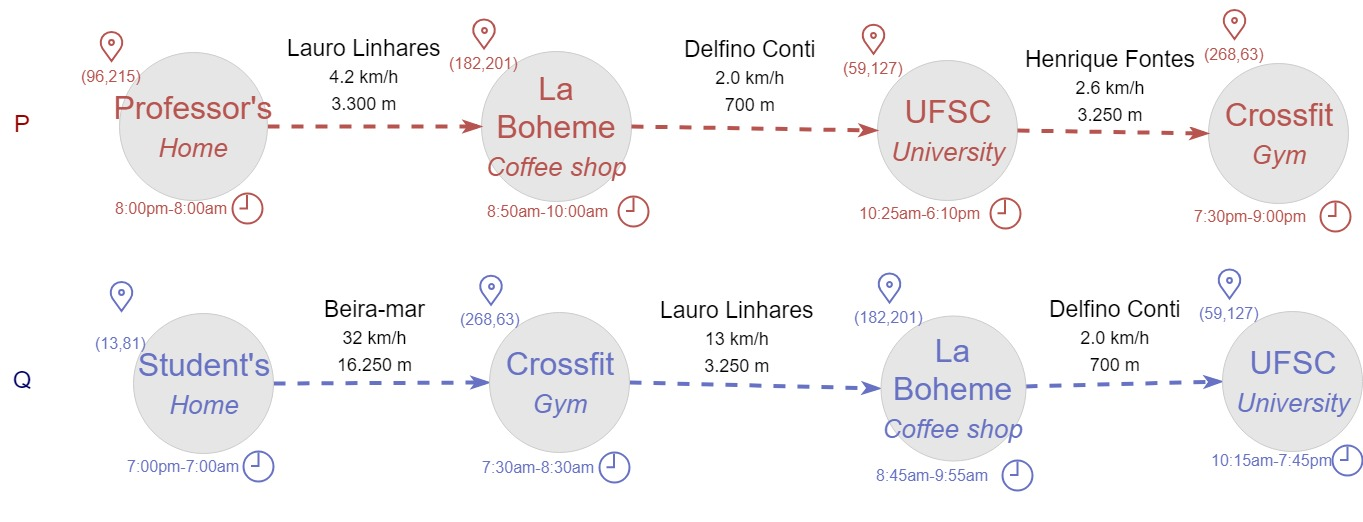
\includegraphics[width=0.95\textwidth]{Related_Works/Semantic_trajectories.jpg}
\caption{\label{fig:related_semantic_trajectories}Two semantic trajectories $P$ and $Q$}
\end{figure}

Answering this kind of question is important in several applications. In car sharing systems, for instance, the origin and destination of the trip is important, but the path followed between the origin and destination is important as well, in order to find ride intersection. In public transportation systems, both bus stops and streets must be known to propose new bus lines. In traffic management applications, the moves between spatial regions must be used to detect traffic jams. In commercial applications, to discover the most effective product promoters or vendors, it is necessary to know the sequence of visited places, the routes followed between places, and how long were both stay at a place and the moves between places, since the objective of the company is to maximize the duration of a stop and minimize the displacement between stops.

%Tanto stops quanto moves podem ser conter vários tipos de informações, como no exemplo da Figura 3, onde os stops possuem a posição do centróide do stop, o intervalo de tempo que o indivíduo permaneceu no stop, assim como o tipo e nome do local onde o stop ocorreu. Os \emph{moves} por sua vez possuem outras informações, como por exemplo o nome da rua por onde o indivíduo trafega, a velocidade média com que o indivíduo se desloca e a distância total percorrida durante o \emph{move}. No trabalho de Furtado já é levado em consideração que os elementos possuam múltiplas dimensões de dados. Só que somente os \emph{stops} são considerados, fazendo com que a medida considere que todos os elementos da trajetória possuam os mesmos tipos de informação, os mesmos atributos. Isto não é válido para trajetórias semânticas, a medida que elas são definidas como uma sequência de \emph{stops} e \emph{moves}, onde tanto os \emph{stops} quanto os \emph{moves} são elementos distintos, com atributos diferentes. Isto faz com que uma trajetória semântica seja uma sequência heterogênea de elementos, onde tanto os elementos \emph{stop} são homogêneos quanto aos atributos contidos, quanto os elemtnos \emph{move} também são homogêneos entre si.

\hl{Both \emph{stops} and \emph{moves} may contain various types of information, as in the example in Figure 3, in which the \emph{stops} have the position of the \emph{stop} centroid, the time interval that the individual stayed in the \emph{stop}, as well as the type and name of the place where the \emph{stop} occurred. The \emph{moves} in turn have other information, such as the name of the street where the individual travels, the average speed in which the individual moves and the total traveled distance. The MSM proposed by Furtado already considers trajectory elements with multiple dimensions, but only the \emph{stops} are considered, and it is assumed that all elements (the stops) have the same types of information/attributes. In other words, all trajectory elements must have homogeneous dimensions, what is not the case for semantic trajectories defined as a \emph{stops} and \emph{moves}, where both \emph{stops} and \emph{moves} are distinct elements, with heterogeneous dimensions. This makes a semantic trajectory an heterogeneous sequence of elements, with \emph{stops} having a set of information to describe itself and \emph{moves} having another set of information.}

In this thesis we propose a new semantic trajectory similarity measure that extends MSM proposed in \cite{Furtado:TGIS12156} to support both \emph{stops} and \emph{moves}. Our approach considers the sequence of the \emph{stops} and supports different semantics for the \emph{moves}. 
In summary, we make the following contributions:
(i) we propose a new similarity measure for multidimensional sequences treating elements with heterogeneous dimensions; (ii) the semantic similarity measure considers both \textit{stops} and \textit{moves}, as well as, their space, time, and semantic information; (iii) we evaluate the proposed measure with experiments over real data, comparing our proposal to both semantic and raw trajectory similarity measures.

The rest of this article is organized as follows: Section \ref{sec:related} presents the related works. Section \ref{sec:proposed_measure} presents the proposed similarity measure with a running example. Section \ref{sec:experiments} presents experiments over real trajectory data, and Section \ref{sec:conclusions} concludes the thesis.

\section{Related works} \label{sec:related}
In this section we present a review on trajectory similarity measures. It is organized as follows: Section \ref{sec:related_raw} presents measures for raw trajectory similarity; and Section \ref{sec:related_semantic} presents measures for semantic trajectory similarity.

\subsection{Raw trajectories} \label{sec:related_raw}
Over the last years, many similarity measures for trajectories were proposed with focus on raw trajectories. A raw trajectories is a discrete representation of the movement of an object that can be defined as a time-ordered finite sequence of space-time points, as formalized in Definition \ref{def:raw_trajectory}. 

\begin{definition} \label{def:raw_trajectory} A raw trajectory is a time-ordered sequence of points in the form T = $<p_1,...,p_n>$ where each point p\textsubscript{k} $\in$ T is a tuple p\textsubscript{k} = (x,y,t), where x,y represent the spatial location of the moving object at a time instant t.
\end{definition}

In the following we describe several trajectory similarity/distance measures. In order to help the understanding, we provide some examples, computing similarity/distance scores using trajectories $P$ and $Q$, as illustrated by Figure \ref{fig:related_trajes}. The spatial coordinates are annotated next to the trajectory points and we consider the time instants as the index associated in each point. For instance, the point \emph{s1} of trajectory $P$ is located at the coordinates $(6,39)$ at time instant $1$.

\begin{figure}[h]
\centering
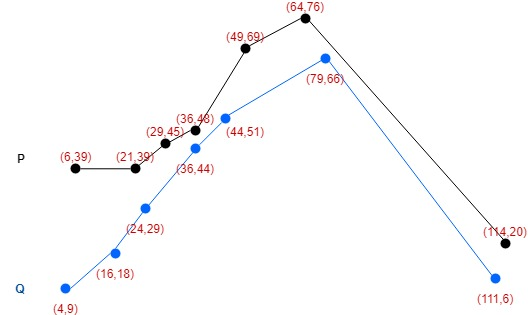
\includegraphics[width=0.85\textwidth]{Related_Works/related_trajes.jpg}
\caption{\label{fig:related_trajes}Two raw trajectories $P$ and $Q$}
\end{figure}

Throughout this section, we use a set of symbols to denote hypothetical trajectories. Table \ref{tab:symbols} summarizes the symbols used in this section.

\begin{table}[!h]
    \centering
    \begin{tabular}{c|c}
         Symbol & Meaning  \\
         \hline
         $P$ and $Q$ & Two trajectories \\
         $m$ and $n$ & Points count of $P$ and $Q$ trajectories respectively \\
         $x,y$ & Spatial coordinates \\
         $dist()$ & Distance function
    \end{tabular}
    \caption{Symbol meanings}
    \label{tab:symbols}
\end{table}

An early proposed distance measure is \emph{Dynamic Time Warping} (DTW) \cite{berndt1994using}, developed for time-series. DTW is used to find the best match between the points of two time-series independent of their sizes. It creates a matrix with all possible pairs of points of the time-series with the pairwise distances as the entries.. %\textcolor{red}{e sem mais de uma dimensao? deves dizer para quais dimensoes faz e se faz para cada uma como junta depois}
The total distance between two trajectories is given by the sum of the entries of the minimum contiguous path in the matrix. Because DTW sums the distances between all points, it tends to be sensitive to noise. For example, when a time-series $P$ has a point that is significantly distant from all points of the time-series $Q$, even if all the other points of $P$ and $Q$ are close, their distance will be dominated by the distant point, adding noise to the analysis. A recursive formalization of DTW is presented in Equation \ref{func:DTW}.

%\textcolor{red}{definicao sem explicar o que é cada letra nao faz sentido, ningume vai entender. Explicar as letras}

\begin{equation}
%\scriptsize
\label{func:DTW}
  DTW(P, Q) = 
  \begin{cases} 
      0 & \text{if } m = n = 0\\ 
      \infty & \text{if } m = 0 \text{ or } n = 0\\ 
      dist(p_1, q_1) + min(DTW(<p_2...p_m>,<q_2...q_n>), & otherwise\\
      DTW(<p_2...p_m>, Q), DTW(P, <q_2...q_n>)) &
  \end{cases}
\end{equation}

Despite being a distance measure for uni-dimensional time-series, DTW can handle with raw trajectory data such as spatial coordinates and temporal information because of its numerical nature. 
The \emph{Multidimensional DTW} (MD-DTW) \cite{ten2007multi} extends DTW for dealing with trajectories whose elements have more than one dimension. MD-DTW normalizes the distance in the different dimensions and then creates a matrix with entries as the sum of the distances in all dimensions. Finally, it runs DTW over the matrix and finds the minimum contiguous path.

Figure \ref{fig:related_trajes_wDF_DTW} (left) illustrates the computation of MD-DTW between trajectories $P$ and $Q$. Its distance is calculated as the sum of the minimum contiguous path between points of $P$ and $Q$, i.e. the sum of all dashed lines, resulting in a distance of $MD-DTW(P, Q) \approx 123$.
%\textcolor{green}{conversando com o EAMON, me parace que o DTW e todas as suas extensoes foram desenvolvidas para time-series, e nao para trajetorias, e tratam atributos numericos, e nao categoricos. Entao talvez pudesse agrupar todos estes dtw e falar isso}

%In a similar approach, \cite{Shokoohi-Yekta2017} proposes a \emph{adaptive DTW} (DTWa) to multidimensional data, focused in classification problems. Its adaptive approach is based on how the distances on all dimensions are integrated, if a \emph{dependent} (DTWd) or an \emph{independent} (DTWi) way \textcolor{red}{explicar essa dependencia e independencia}. The DTWd approach is similar of MD-DTW, where all distance matrixes are computed, its entries are normalized, summed, and stored in a new distance matrix, which is used to calculate DTW distance.  On the dependent way (DTWd), all distance matrixes are normalized, but instead sum the entries, the DTW is performed over all matrixes, the distance of each dimension is calculated, and then its distances are summed, resulting in the DTWi distance. The decision of which approach is more reliable is made by processing a trajectory over a training data set and based on which approach is more precise over the train data, \textcolor{red}{frase seguinte parece nao ter conexao com a anterior} it is choose to classify the trajectory.

Ding in \cite{Ding:2008:ESJ:1440463.1440989} proposes \emph{w-constrained discrete Fr{\'e}chet Distance} (wDF), which extends the Discrete Fr{\'e}chet distance \cite{eiter1994computing} by adding a temporal window, in order to consider only the pairs of points that are within a given \emph{w} time window. The distance between the trajectory points is directly calculated by a continuous distance function (e.g. Euclidean distance), leading the measure to be sensitive to noise. Indeed, this measure makes the assumption that the two trajectories have the same number of points, making point interpolation when necessary.

The wDF distance is given by the minimum distance of all possible time windows over two trajectories, where the distance of each window is the maximum distance between all pairs of points of $P$ and $Q$  inside the window, as shown in Equation \ref{func:match_wDF}.

\begin{equation}
\label{func:match_wDF}
  wDF(P, Q) = min(\forall_{i,j=0}max(dist(P_i, Q_j))) \Rightarrow i \leq j + w \land
  j \leq P_{length} - w
\end{equation}

Figure \ref{fig:related_trajes_wDF_DTW} (right) shows trajectories $P$ and $Q$ and a \emph{w} time-window sample. The wDF distance between the trajectories is computed as the maximal distance found among all \emph{w}-constrained time-windows. As the time-window shifts over trajectories, the maximal distance between their points is computed, using the Euclidean distance. In the example of Figure \ref{fig:related_trajes_wDF_DTW} (right), the wDF distance is $wDF($P$, $Q$) = euclidean((38,51), (29,38)) \approx 4$.

\begin{figure}[h]
\centering
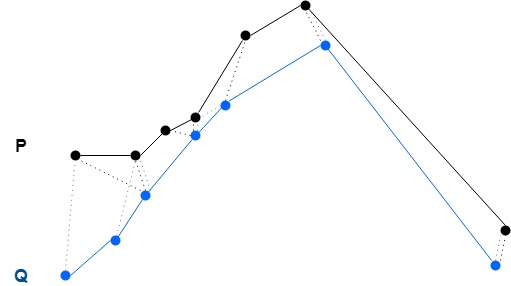
\includegraphics[width=0.45\textwidth]{Related_Works/related_trajes-DTW.jpg}
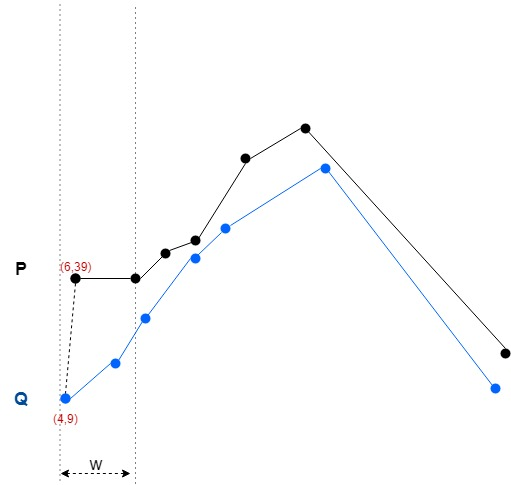
\includegraphics[width=0.45\textwidth]{Related_Works/related_trajes-wDF.jpg}
\caption{\label{fig:related_trajes_wDF_DTW}(left) MD-DTW score is the sum of minimum distance between all points from smaller trajectory to longer. (right) wDF score is the minimal distance of all maximal distances between two points within the given time window \textit{w}}
\end{figure}

Vlachos \cite{vlachos2002discovering} proposed the \emph{Longest Common Subsequence} (LCSS) for raw trajectory similarity measuring, considering the spatial distance between two points. In Vlachos' work two points \textit{match} if the distance between them is less than a given \textit{threshold} $\epsilon$, as can be seen in Equation \ref{func:match_LCSS}. LCSS reduces the effect of noisy data by quantifying the similarity between two elements to binary values: 1 if the elements match, 0 otherwise. The longer the common subsequence of point matches between two trajectories, the more similar they are. 

%\textcolor{blue}{explicar as letras das formulas. Se voce usar sempre as mesmas letras para todas as formulas voce poderia fazer uma frase no inicio colocando uma tabelinha com as letras e dizendo o que significam, dai durante as explicacoes vc so explicaria o que muda nas formulas}

\begin{equation}
%\scriptsize
\label{func:match_LCSS}
  match(p, q) = 
  \begin{cases} 
      true & dist(p_x, q_x)  \leq \epsilon\\ 
        &            \text{and } dist(p_y, q_y)  \leq \epsilon\\
      false & otherwise
  \end{cases}
\end{equation}

A recursive formalization of LCSS is presented in Equation \ref{func:LCSS}.

\begin{equation}
%\scriptsize
\label{func:LCSS}
  LCSS(P, Q) = 
  \begin{cases} 
      0 & \text{if } m = n = 0\\ 
      1 + LCSS(<p_2...p_m>,<q_2...q_n>) & \text{if } match(p_1, q_1)\\
      max(LCSS(<p_2...p_m>, Q), LCSS(P, <q_2...q_n>)) & otherwise
  \end{cases}
\end{equation}

As the LCSS distance is the sum of all matched points between two trajectories, to be used as a similarity measure it needs to be normalized between 0 and 1. The LCSS similarity score is given by the size of the longest common subsequence ($LCSS(P, Q)$) over the size of the shortest trajectory, i.e., $\dfrac{LCSS(P, Q)}{min(m, n)}$.
Figure \ref{fig:related_trajes_EDR_LCSS} (left) shows the matching of points of trajectories $P$ and $Q$ considering a 15-meter threshold. The LCSS similarity score of $P$ and $Q$ is the total of matched points (solid black) normalized by the size of the shortest trajectory, $LCSS($P$, $Q$) = \dfrac{5}{7} \approx 0.71$.

A drawback of LCSS is it subsequence specificity, causing a inability to take into account gaps of any size in the trajectory. Figure \ref{fig:related_trajes_PQR} shows three trajectories $P$, $Q$, and $R$, with 3, 4, and 5 points, respectively. The LCSS similarity of $P$ and $Q$ is $LCSS(P, Q) = 1$, while the similarity of $P$ and $R$ is also $LCSS(P, R) = 1$, even though two points of $R$ do not match any points of $P$ and only one point of $Q$ does not match a point of $P$.


\begin{figure}[h]
\centering
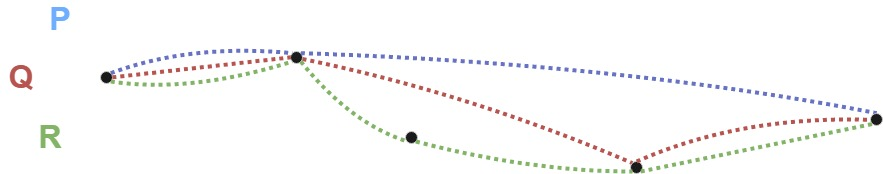
\includegraphics[width=0.9\textwidth]{Related_Works/related_trajes_PQR.jpg}
\caption{\label{fig:related_trajes_PQR}Trajectories $P$, $Q$ and $R$ share 3 points, while trajectories $Q$ and $R$ share 4 points.}
\end{figure}


Chen in \cite{Chen:2005:RFS:1066157.1066213} proposes the Edit Distance on Real sequence (EDR), another similarity measure for raw trajectories. EDR calculates the distance between two trajectories by computing the edit distance between their spatial points. The edit distance between two trajectories is given by summing the distance between their points quantified as 1 if both spatial points do not match, and 0 when they match (the \emph{subcost}). Using this approach, EDR solves the problem of the gaps in LCSS, by taking into account points that do not match. However, to enforce a match between two points EDR requires that their distance is below a given threshold in all dimensions.

A recursive  formalization of EDR is presented in Equation \ref{func:EDR}.

\begin{equation}
%\scriptsize
\label{func:EDR}
  EDR(P, Q) = 
  \begin{cases} 
      0 & \text{if } m = 0\\ 
      0 & \text{if } n = 0\\ 
      min(EDR(<p_2...p_m>,<q_2...q_n>) + subcost, & otherwise\\
      EDR(<p_2...p_m>, Q) + 1, EDR(P, <q_2...q_n>) + 1) &
  \end{cases}
\end{equation}

The EDR similarity score is given by the inverse of the number of non-matched points over the size of the longest trajectory, i.e., $1 - \dfrac{EDR(P, Q)}{max(m, n)}$. In the case of Figure \ref{fig:related_trajes_EDR_LCSS} (right), trajectories $P$ and $Q$ only non-match in 2 of their points (solid black) when using a threshold of 15 meters. The EDR similarity score of $P$ and $Q$ is the inverse of the total of non-matched points over the size of the longest trajectory, $EDR($P$, $Q$) = 1 - \dfrac{2}{7} \approx 0.71$.

Comparing the trajectories from Figure \ref{fig:related_trajes_PQR} with EDR, the similarity of $P$ and $Q$ is $EDR(P, Q) = 0.75$ and the similarity of $P$ and $R$ is $EDR(P, R) = 0.60$. These similarity scores show that EDR is robust to gaps in trajectories, by giving distinct similarity scores for trajectories of different sizes, solving the drawback of LCSS. Moreover, EDR maintains the robustness to noise of LCSS by using a threshold value in all dimensions.

\begin{figure}[h]
\centering
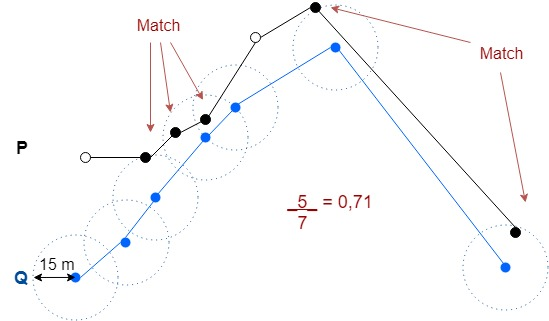
\includegraphics[width=0.45\textwidth]{Related_Works/related_trajes-LCSS.jpg}
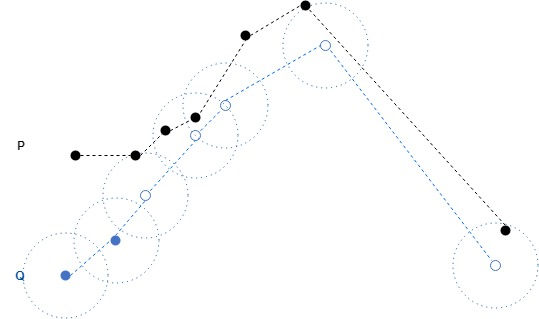
\includegraphics[width=0.45\textwidth]{Related_Works/related_trajes-EDR.jpg}
\caption{\label{fig:related_trajes_EDR_LCSS}(left) LCSS similarity score is the number of matched points normalized by the size of shortest trajectory. (right) EDR distance score is the number of non-matched points normalized by the size of largest trajectory, subtracted by 1.}
\end{figure}

Furtado proposes the \emph{Uncertain Movement Similarity} (UMS) in \cite{Furtado-UMS-2018}. UMS is a parameter-free similarity measure for raw trajectories. UMS was designed exclusively for raw trajectories, using only the spatial dimension. The main contribution of UMS is the elimination of parameters for similarity measuring, by defining a dynamic spatial threshold that is computed automatically according to the distance between the trajectory points. As a consequence, it solves the problem of irregular distribution of trajectory points. UMS represents trajectories as a sequence of movement ellipses, covering the space between two sampled trajectory points. The size of each ellipse is defined dynamically, using the \emph{Approximate Upper Bound} (AUB) function, also proposed in their work. By using a dynamic ellipse size,  UMS avoids the definition of a radius of fixed size, which is a problem for real applications where the sampling rate can be low and/or irregular, since it is very difficult to estimate such parameter from the user point of view.

UMS measures the similarity of two elliptical trajectories by analyzing three premises:
\begin{itemize}
  \item \textit{Alikeness}: the shapes formed by the union of ellipses look alike;
  \item \textit{Shareness}: the space covered by both ellipses have a greater common area;
  \item \textit{Continuity}: the ellipses order represents moving objects traveling continually in the same direction.
\end{itemize}

Figure \ref{fig:related_trajes_UMS} shows the trajectories $P$ and $Q$ represented as two elliptical trajectories according to UMS. As shown, both elliptical trajectories have some similarity in their ellipses, with the elliptical shapes looking alike (\emph{alikeness} = 0.49), sharing a common area, mainly in their last ellipses (\emph{shareness} = 0.31), and keeping some order in the ellipses sequence (\emph{continuity} = 0.49). The UMS distance is calculated as $UMS($P$, $Q$) = \dfrac{alikeness + shareness}{2} * continuity$, resulting in an UMS similarity score of $0.19$ for $P$ and $Q$, indicating that both the trajectories have some commonalities but in the majority they are dissimilar.

\begin{figure}[!h]
\centering
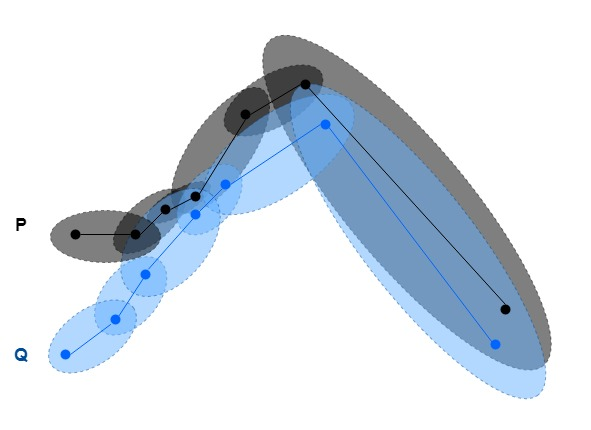
\includegraphics[width=0.75\textwidth]{Related_Works/related_trajes-UMS.jpg}
\caption{\label{fig:related_trajes_UMS}UMS similarity score is given by: i) the shape \textit{alikeness} of ellipses; ii) the \textit{shared} area of ellipses; and iii) the \textit{continuity} of points inside ellipses}
\end{figure}

\subsection{State of Art on Semantic trajectories} \label{sec:related_semantic}
Traditionally a trajectory is represented as stated in Definition \ref{def:raw_trajectory}, i.e., a time-ordered sequence of spatial points. Alvares \cite{alvares2007model} and Spaccapietra \cite{Spaccapietra:2008:CVT:1347466.1347785} proposed a new representation for trajectories, defining a trajectory as a time-ordered sequence of \emph{stops} and \emph{moves}, where the \emph{stops} are the more relevant part of the trajectory.
In this work, we formally define semantic trajectory, considering its sequence of stops and moves, which is an enriched extension of the definition presented in \cite{Spaccapietra:2008:CVT:1347466.1347785}:

\begin{definition}
\label{def:semantic_trajectory}
A semantic trajectory  $SemTraj=\langle s_1, m_1, s_2, m_2, s_3,m_3, ...., s_n, m_n, s_{n+1} \rangle$ is a time ordered sequence of stops and moves, where each stop $s_i$ has a set of attributes $\{d_{a1}, d_{a2}, ...d_{aq}\}$ characterizing it according to q-dimensions, and each move $m_j$  has a set of attributes $\{d_{b1}, d_{b2}, ...d_{br}\}$  characterizing it according to r-dimensions. 
\end{definition}    

For this new definition of trajectory, the definition of new semantic-aware similarity measures are necessary. These new measures may analyze, besides the semantic information, any other information about the trajectory, as for instance the temporal duration of \emph{stops} and \emph{moves}, the spatial source point of these elements, average speed in \emph{moves} and so on.

In the following we describe a few semantic similarity measures, as well as theirs limitations and applications. In order to help understand, we provide some examples, computing similarity scores using trajectories $P$ and $Q$, as previously illustrated in Figure \ref{fig:related_semantic_trajectories}. These trajectories are annotated with the spatial coordinates of the \emph{stops} centroids, the time interval of each \emph{stop}, the name and type of place where \emph{stop} takes place, the name of the main street where \emph{move} occurs, and the travelled distance and average speed during the \emph{move}.

%\textcolor{blue}{comecar a seçao com uma historia, falando que pesquisa em trajetorias semanticas eh mais recente e que os metodos sao limitados. Penso que precisas distinguir quem faz realmente similaridade e quem faz outra coisa. O DTW e seuas extensoes deve ser eliminado desta seçao}
An early similarity measure considering semantic trajectories is Common Visit Time Interval (CVTI) proposed in \cite{Kang:2009:SMT:1529282.1529580}. It was proposed as a measure, integrating the semantic information of the elements with the temporal dimension. It finds the Longest Common Subsequence of two semantic trajectories in which both semantic information is the same and it exists a time intersection between elements. 

CVTI is strongly based on LCSS, thus presenting the same drawback of LCSS: the inability to penalize gaps of any size in the trajectory, as illustrated in Figure \ref{fig:related_trajes_PQR}. Although CVTI uses different data dimensions, the measure is not extensible for other data dimensions associated with \emph{stops} and \emph{moves}.

Figure \ref{fig:related_trajes_CVTI_MSTP} (left) shows the computing of the CVTI similarity score. CVTI finds the Longest Common Subsequence (LCSS) of elements between both trajectories $P$ and $Q$, considering both the semantic and time dimensions. Here, the LCSS of $P$ and $Q$ are $LCSS_{CVTI}(P, Q) = 5$. The similarity score of CVTI is given by the computed LCSS over the size of the shortest trajectory, i.e., $CVTI(P, Q) = \dfrac{LCSS_{CVTI}(P, Q)}{min(m, n)}$. In the example of Figure \ref{fig:related_trajes_CVTI_MSTP}, the CVTI similarity score is given by $CVTI(P, Q) = \dfrac{5}{7} \approx 0,71$.

In \cite{Ying:2010:MUS:1867699.1867703} the measure \emph{Maximal Semantic Trajectory Pattern Similarity} (MSTP) was proposed. It identifies the Longest Common Sequence (LCS) between two semantic trajectories, which are sequences of labels describing the types of places such as $<Scholl, Park, Cinema>$. MSTP differentiates from LCSS because it computes a ratio between each trajectory and their common pattern, i.e. the sequence of places visited by both trajectories. The average ratio is used to compute the similarity score, avoiding the drawback of LCSS that does not differentiate matching gaps of different sizes. A limitation of this approach is that it focuses only in semantic similarity, not being extensible for multiple dimensions, as time and spatial dimensions.

Figure \ref{fig:related_trajes_CVTI_MSTP} (right) shows how MSTP computes the similarity score between two trajectories. First of all, MSTP needs to mine the frequent pattern from each user. In this figure there are 4 distinct patterns, each of them with a distinct background color. After, MSTP identifies the patterns present in both trajectories and computes the LCS distances of each pattern with the actual semantic trajectory. Then, it computes a ratio between the LCS distance score and the length of each trajectory, i.e., $ratio(LCS(P, Q), P) = \dfrac{\sum\limits_{j=0}^{m} \sum\limits_{j=0}^{|LCS(P,Q)|} P_i \cap LCS_j}{|P|}$.

Finally, the sum of the \emph{ratios} for $P$ and $Q$ is divided by the sum of the pattern count of $P$ and $Q$, resulting in the final similarity score.

In the example of Figure \ref{fig:related_trajes_CVTI_MSTP}, the similarity score of trajectories $P$ and $Q$ is given by $MSTP(P, Q) = \dfrac{ratio_P + ratio_Q}{|Patterns_P| + |Patterns_Q|} = \dfrac{2 + 2}{2 + 2} = 1$, indicating that the trajectories are identical, because they have all patterns found in both trajectories.

\begin{figure}[h]
\centering
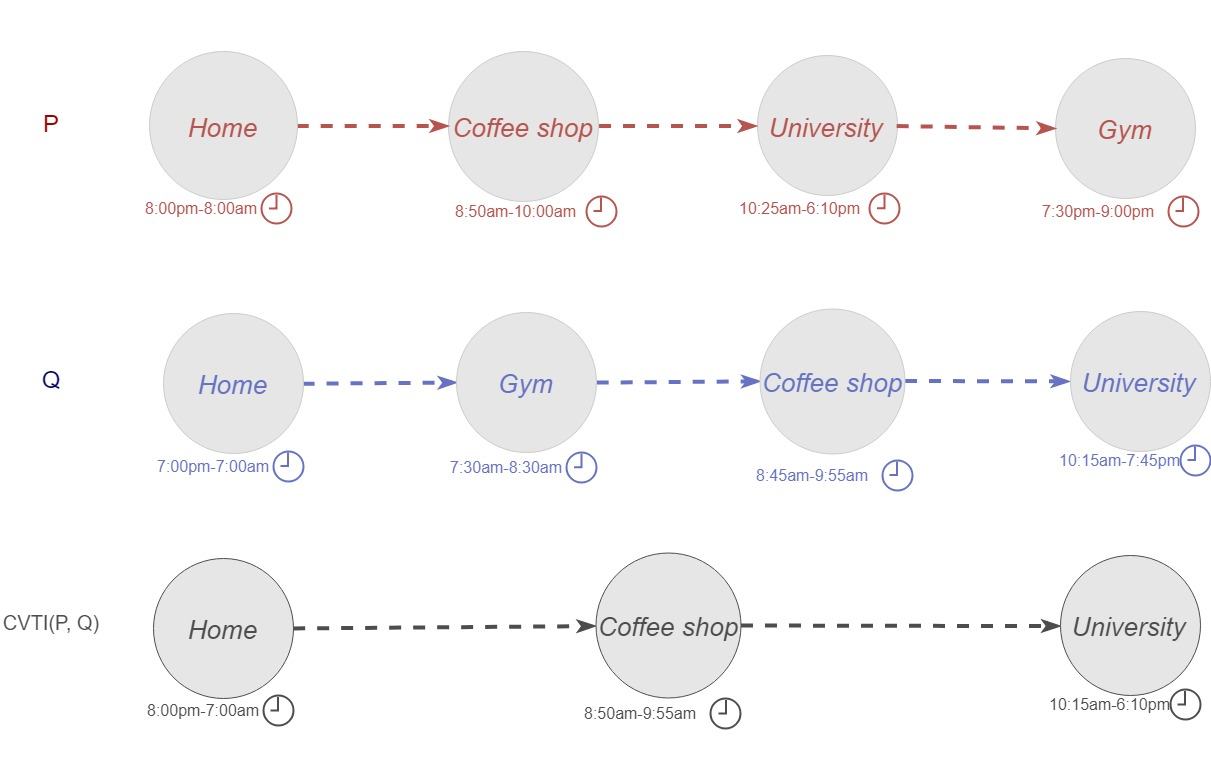
\includegraphics[width=0.45\textwidth]{Related_Works/Semantic_Trajectories_(CVTI).jpg}
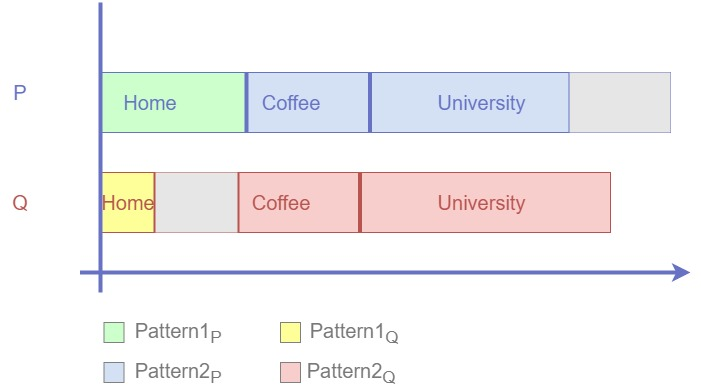
\includegraphics[width=0.45\textwidth]{Related_Works/Semantic_Trajectories_(MSTP).jpg}
\caption{\label{fig:related_trajes_CVTI_MSTP}(left) CVTI similarity score is the longest common subsequence with time intersection between two trajectories. (right) MSTP similarity score is based on the longest common sequence of patterns.}
\end{figure}

%In \cite{Ying:2010:MUS:1867699.1867703} the measure \emph{Maximal Semantic Trajectory Pattern Similarity} (MSTP) was proposed, which despite being a measure for semantic trajectories is not able to handle multiple data dimensions. Moreover, as MSTP essentially works with the frequency at which stops are visited, it is not able to represent moves between stops, ignoring all information about movement.

The work of Liu\cite{Liu:2012:SMM:2442968.2442971} proposed a semantic similarity measure that combines two distances: geographic and semantic. The geographic distance considers three aspects: the distance between the centroids of trajectories, the difference in the length of the trajectories, and the cosine similarity of the directions of subtrajectories. The semantic distance is based on LCSS to find the longest common subsequence of types of places that were visited by the individual. Their approach uses speed variation to split trajectories into subtrajectories, and then the cosine distance is computed between subtrajectories. Limitations of this approach include: i) sensibility to noise in the geographic distance; ii) the time distance is not considered in the distance calculation; and iii) the prevalence of the geographic distance, i.e. two trajectories are similar only if they are similar in space.

\begin{figure}[h]
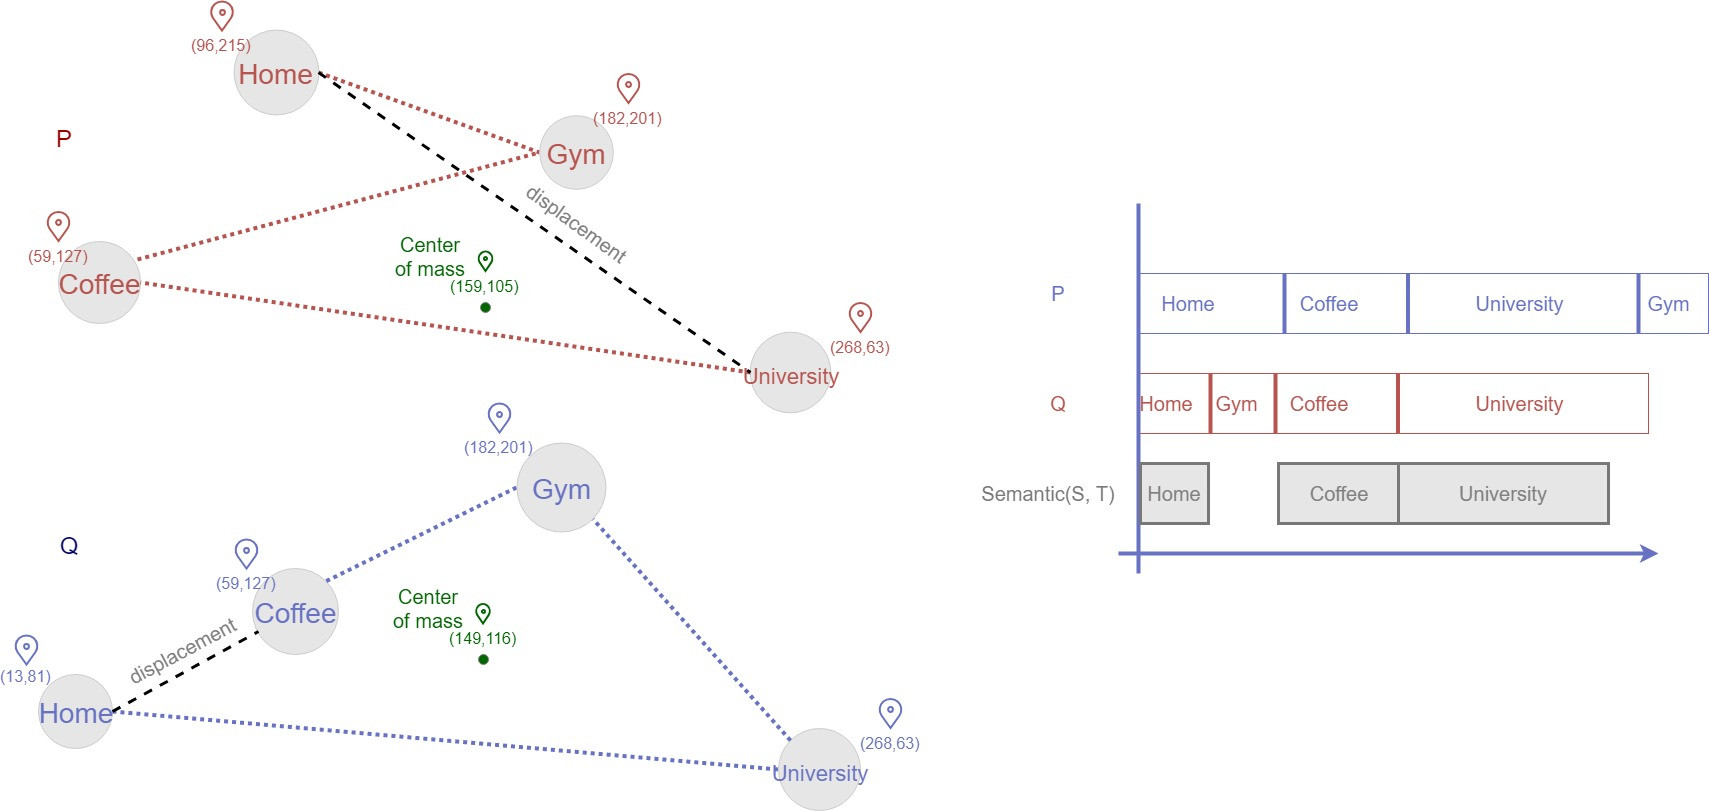
\includegraphics[width=0.9\textwidth]{Related_Works/Semantic_Trajectories_(Liu).jpg}
\caption{\label{fig:related_trajes_Liu}(left) Liu's work compute spatial similarity score based on center of mass and the displacement of trajectories. (right) The semantic similarity score is strongly based on LCSS.}
\end{figure}

Figure \ref{fig:related_trajes_Liu} presents the basic elements for computing the similarity measure proposed by Liu. The image on the left shows the displacement and the center of mass of both trajectories $P$ and $Q$. On the right side, the computation of the semantic similarity is illustrated. As the centroids of both trajectories and their traveled distances are close, plus their great similarity in semantic dimension, both trajectories are very similar by Liu's similarity measure.

\emph{Maximal Travel Match} (MTM)\cite{Xiao:2010:FSU:1869790.1869857} analyzes trajectory similarity in the semantic dimension constrained by the time dimension. In order to do that, it proposes a semantic similarity measure that takes into account the semantic of the visited place (e.g., restaurant, university etc.), the sequence of the visited places, the traveled time between places, and the frequency that a place was visited. Two trajectories are more similar if they visited places of the same type, in the same order with similar travel times, according to a time threshold. Limitations of this approach include: i) two semantic trajectories are similar only if they visit the places in the same order; ii) the space dimension is not considered; and iii) MTM measures the similarity considering the whole dataset in order to obtain the frequency of the visited places, what makes the result dependent of the other trajectories in the dataset.

%The distance measure Dynamic Time-Warping adaptive (DTWa) proposed in \cite{Shokoohi-Yekta2017} extends the classical DTW \cite{berndt1994using} distance measure by allowing two data series to have their distance measured using multiple data dimensions. The input of DTWa must be a sequence of points with homogeneous dimensions, so having similar problems as previous measures.

In the work of \cite{Furtado:TGIS12156}, the MSM (Multidimensional Similarity Measuring) measure was proposed, working with multiple dimensions. MSM was designed to handle multidimensional sequences, in which each dimension is independent and each dimension should have its own distance function, i.e., all elements must be homogeneous. MSM is a match-based similarity measure, which means that for each dimension there is a threshold value defining if two elements match or do not match. Limitations of this approach include: i) the elements homogeneity allows MSM to handle \textit{stops} only, since \textit{stops} and \textit{moves} have distinct attributes, and ii) the order of the elements is not taken into account during the similarity calculation.

Cai in \cite{CaiLee2016} proposed a measure that combines the strategies of LCSS \cite{vlachos2002discovering} and MSM\cite{Furtado:TGIS12156} for semantic trajectories. It finds the longest common subsequence between two semantic trajectories. The difference to LCSS is that it does not require the matching in all dimensions, and it does separate the dimensions in two types: compulsory and optional. While all dimensions of the first category should be similar for two elements to match, the optional ones are used only to increase the score, with of their weights being defined in a similar way to MSM.


\section{The Proposed Measure: SMSM} \label{sec:proposed_measure}
In this section we present a novel similarity measure to consider both stops and moves of semantic trajectories, called SMSM (\textit{Stops and Moves Similarity Measure}). The idea behind SMSM is a measure that overcomes the strictness of LCSS and EDR by allowing partial order and dimension matching, and the limitations of MSM by considering both stops and moves.
%Before we introduce the concepts related to the new measure, we formally define semantic trajectory, considering its sequence of stops and moves, which is an enriched extension of the definition presented in \cite{Spaccapietra:2008:CVT:1347466.1347785}:


%\begin{definition}
%\label{def:semantic_trajectory}
%A semantic trajectory  $ST=\langle s_1, m_1, s_2, m_2, s_3,m_3, ...., s_n, m_n, s_{n+1} %\rangle$ is a time ordered sequence of stops and moves, where each stop $s_i$ has a set of %attributes $\{d_{s1}, d_{s2}, ...d_{sq}\}$ characterizing it according to q-dimensions, and %each move $m_j$  has a set of attributes $\{d_{m1}, d_{m2}, ...d_{mr}\}$  characterizing it %according to r-dimensions. 
%\end{definition}

In this work we assume that a semantic trajectory starts and ends with a stop, otherwise we transform the first and/or the last point of the trajectory in a stop. In the following section we present the new concepts and the definition of the proposed similarity measure SMSM.
\subsection{Basic Concepts and the Proposed Measure}

Stops and moves by definition are different and heterogeneous trajectory elements. A stop may have a spatial position, a start and end time, a category, or a set of attributes related to the category (e.g. Category hotel, stars, rate, price), etc. A move always starts and ends in a stop and may be characterized by different attributes as average speed, traveled distance, sequence of streets, duration, the sequence of raw points, etc. These attributes are defined according to the needs of the application. 

In order to deal with these heterogeneous elements (stops and moves), we introduce the concept of \emph{movement element}. A movement element is a new representation that is not treated by other measures, mainly MSM, which supports only stops. Indeed, MSM does not consider the order of trajectory elements, while in our approach we preserve the sequence of both stops and moves in a movement element.

\begin{definition}
\label{def:movement_element}
A movement element  $e=(stopS, move, stopE)$ is a tuple formed by a start stop $stopS$, the $move$ between $stopS$ and  $stopE$, and the end stop $stopE$, where stopS and stopE are two consecutive stops.
\end{definition}


Hereafter we will consider a semantic trajectory as a sequence of \textit{homogeneous movement elements}, as follows: 
$ST=\langle e_1=(s_1,m_1,s_2), e_2=(s_2,m_2,s_3), ..., e_n=(s_n,m_n,s_{n+1}) \rangle$.

Notice that we define a movement element as a homogeneous trajectory part, but they will be analyzed separately later in our measure.
This structure will be used for the proposed similarity measure, where one trajectory will be compared with another one based on their movement elements.



We analyze the similarity of a movement element $a\in A$ with another movement element $b\in B$, where A and B are semantic trajectories, in two parts: their stops and their moves.The basis for measuring the similarity of these two parts is the \emph{match} function, given in Equation \ref{func:match1}. The function returns 1 if the distance between an attribute (also called dimension) of two movement elements is less than a given threshold \emph{maxDist}, and zero otherwise. This function is used for measuring the distance of all dimensions of both: the stops and the moves.

\begin{equation}
%\scriptsize
\label{func:match1}
  match_i(a, b) = 
  \begin{cases} 
      1 & dist_i(a, b) \leq maxDist_i \\
      0 & otherwise
  \end{cases}
\end{equation}

To compute a total score for two movement elements $a$ and $b$ we define the function \emph{score(a,b)} in Equation \ref{func:score1}. We consider a score for the stops (scoreStop) and a score for the move (scoreMove). As the degree of importance of stops and moves can vary from one application to another, we also define a weight for both stops and moves. 


\begin{equation}
%\scriptsize
\label{func:score1}
score(a, b) = scoreStop(a, b) * w_{stop} + scoreMove(a, b) * w_{move}  
\end{equation}

where, $w_{stop}$ and $w_{move}$ are the weights of the stops and the moves, respectively, and their sum should be one.

The functions \emph{scoreStop(a,b)} and \emph{scoreMove(a,b)} are defined in Equations \ref{func:scoreStop1} and \ref{func:scoreMove2}, respectively, where $r$ and $q$ are the number of dimensions (attributes) of stops and moves, respectively.


\begin{equation}
%\scriptsize
\label{func:scoreStop1}
%\begin{split}
  scoreStop(a, b) = \sum\limits_{i=1}^r (match_i(a_{stopS}, b_{stopS}) + match_i(a_{stopE}, b_{stopE}))\div 2* w_{i}
%\end{split}
\end{equation}


\begin{equation}
%\scriptsize
\label{func:scoreMove2}
\begin{split}
scoreMove(a, b)  & = 
  \begin{cases} 
      \sum\limits_{i=1}^q match_i(a_{move}, b_{move}) * w_{i} & if matchStops(a, b)\\
      0 & otherwise
  \end{cases}
\end{split}
\end{equation}


The sum of the weights in Equations \ref{func:scoreStop1} and \ref{func:scoreMove2} should be one.
The score of the stops computed according to Equation \ref{func:scoreStop1} is given by the average of all dimension matches of the start and end stops of two movement elements $a$ and $b$. Note in Equation \ref{func:scoreMove2} that the \emph{scoreMove} depends on the function \textit{matchStops(a, b)}.

The function \ref{func:matchStops} presents the computing of the \emph{matchStops(a,b)}. The result of this function is true when the spatial distance between $a_{stopS}$ and $b_{stopS}$ is less than $maxDist$ and the spatial distance between $a_{stopE}$ and $b_{stopE}$ is also less than $maxDist$. This means that a move similarity will be analyzed only when the spatial distance of both $start$ and $end$ \emph{stops} of the movement elements $a$ and $b$ are spatially close. 

\begin{equation}
%\scriptsize
\label{func:matchStops}
\begin{split}
matchStops(a, b)  & = 
  \begin{cases} 
      true & match_{spatial}(a_{stopS}, b_{stopS}) \text{ and } match_{spatial}(a_{stopE}, b_{stopE})\\
      false & otherwise
  \end{cases}
\end{split}
\end{equation}

Figure \ref{fig:move} shows an example of several trajectories with a stop in $A$ and then in  $B$, following three different paths, $P_1$, $P_2$, and $P_3$. One trajectory moves from stop A to stop C, following path $P_4$. As can be seen in the figure, trajectories going from A to B are more similar between them in relation to the trajectory going from A to C.
In real scenarios, this means that if we want to analyze trajectories going, for instance, from France to Italy, we do not need to compare them with trajectories going from France to Spain, since they are moving to different destinations. In the example in Figure \ref{fig:move}, if we are interested in trajectories moving from A to B, we only analyze the moves (paths $P1$, $P2$, and $P3$) of trajectories going from A to B, and these three paths will not be compared with $P4$. In other words, the similarity of the movement elements $<A, P_1, B>$, $<A, P_2, B>$, $<A, P_3, B>$ will be compared among them, and not with the movement element $<A, P_4, C>$.

The function \emph{scoreMove} guarantees a partial order in the similarity analysis, what has not been considered in the MSM measure.

\begin{figure}[h]
\centering
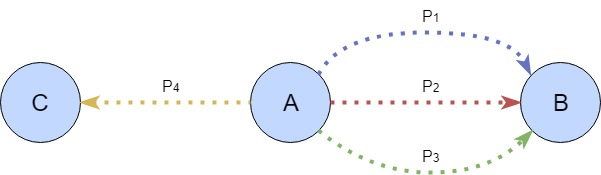
\includegraphics[width=0.75\textwidth]{Images/Toy_trajectories.jpg}
\caption{\label{fig:move} Trajectories moving from region $A$ to region $B$ following the paths (moves) $P_1$, $P_2$, and $P_3$; and trajectories moving from $A$ to C following path $P_4$}
\end{figure}

Having defined the score for stops and moves for comparing movement elements, Equation \ref{func:parity} defines the parity of two semantic trajectories A and B. The parity of A with B is
the sum of the highest score of all the elements $a \in A$ when compared with all the elements of B.
\begin{equation}
\label{func:parity}
parity(A, B) = \sum\limits_{a\in A} \textbf{max}\{\textit{score}(a, b) : b \in B\}
\end{equation}

Finally, we can define the global similarity of two trajectories A and B with $SMSM$. Equation \ref{func:SMSM1} defines the stops and moves similarity measure SMSM(A,B) by the average parity of $A$ with $B$ and of $B$ with $A$.

\begin{equation}
\label{func:SMSM1}
%\scriptsize
\begin{split}
  SMSM(A, B) = 
  \begin{cases} 
      0 & if  |A| = 0 \vee |B| = 0 \\
      \frac{parity(A, B) + parity(B, A)}{|A| + |B|} & otherwise
  \end{cases}
\end{split}
\end{equation}



\subsection{Evaluation over a running example}

In this section we present a running example, comparing SMSM and MSM, since MSM is the closest approach to the proposed similarity measure.
Let us consider the two trajectories shown in Figure \ref{fig:SMSM_examples_PQ}. Trajectory $Q$ represents the daily routine of a professor, that starts his day at the gym in the morning, while trajectory $P$ is the daily routine of a student, that starts his day at a coffee shop. Considering the stop name, the spatial position, and the start and end time of the stop, the student has the following movement behavior: stays at \textit{Home} $((96,215), [8pm-8am])$, than he goes via Edu Vieira street to have breakfast at the \textit{Coffee shop} $((182,201), [8:50am-10am])$, and from there goes via Delfino Conti street to the \textit{University} $((59,127), [10:25am-6:10pm])$, finishing the day moving via Henrique Fontes street to the \textit{Gym} $((268,63), [7:30pm-9pm])$. The professor (trajectory $Q$) goes from \textit{Home} $((13,81), [7pm-7am])$ via Beira-mar avenue jogging at the \textit{Gym} $((268,63), [7:30am-8:30am])$. After he goes to the \textit{Coffee shop} $((182,201), [8:45am-9:55am])$ via Edu Vieira street, and via Delfino Conti reaches the \textit{University} $((59,127), [10:15am-7:45pm])$ to teach his classes until the end of the day. We have two trajectories $P$ and $Q$ with their stops and moves annotated with the category of the place, the spatial information of the visited place, the time of the visit, and the name of the street to represent the move. Both trajectories visit the same places, sharing some streets, but in totally different order.
\begin{figure}[h!]
\centering
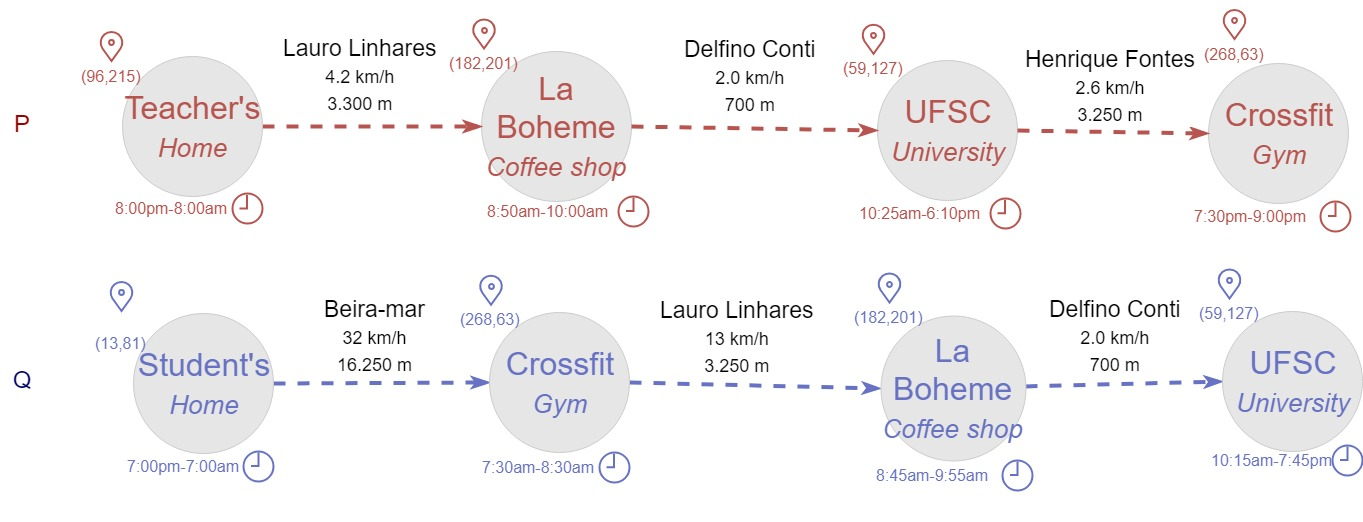
\includegraphics[width=1\textwidth]{Images/Semantic_trajectories.jpg}
\caption{\label{fig:SMSM_examples_PQ} Trajectories $P$ (Student) and $Q$ (Professor)}
\end{figure}


In order to calculate the SMSM similarity value, we first need to construct all movement elements for each trajectory. Table \ref{tab:SMSM_tuples} lists these elements, where each element contains the start stop, the name of the street followed during the move, and the next stop. Notice in this table that the only movement element where the moves will be measured is $<Coffee shop, Delfino Conti, University>$ from trajectory $P$ and $<Coffee shop, Delfino Conti, University>$ from trajectory $Q$, because both start and end stops match.

\begin{table}[h!]
\scriptsize
  \centering
  \begin{tabular}{|c|c|}
  	\hline
		\textcolor{Red}{\textbf{Student (P)}} & \textcolor{Blue}{\textbf{Professor (Q)}}\\
  	\hline
      $<$Home, Edu Vieira, Coffee$>$&$<$Home, Beira-mar, Gym$>$\\
      $<$Coffee, Delfino Conti, University$>$&$<$Gym, Edu Vieira, Coffee$>$\\
      $<$University, Henrique Fontes, Gym$>$&$<$Coffee, Delfino Conti, University$>$\\
  	\hline
  \end{tabular}
  \label{tab:wrong}
  \caption{Movement elements}
  \label{tab:SMSM_tuples}
\end{table}

To measure the distance between two movement elements, we choose the following distance functions for measuring the distance of stop dimensions:
\begin{itemize}
  \item Space: the Euclidean distance between the centroids of the stops;
  \item Time: the time distance of two stops is given by the inverse of the proportion between the intersection of their periods divided by the total period between the minimum starting time and the maximum ending time;
  \item Semantics: the distance is equal to 0 in case of exact match and equal to 1 otherwise.
\end{itemize}
For the sake of simplicity, for the move, in this example we consider only the semantic information, i.e., the name of the followed street, where the distance is equal to 0 in case of exact match of street name and equal to 1 otherwise.

In this running example we use as thresholds \textit{maxDist\textsubscript{space}} = 100 meters and \textit{maxDist\textsubscript{time}} = 0.5, i.e. two stops are said as matched in time when both share half of their period in that stop.
With distance functions and threshold values defined and elements constructed, we use Equation \ref{func:score1} to measure the similarity values between all element dimensions, computing first the match in both start and end stops and if the stops match we compute the match for the move. 

To understand how to measure the movement element similarity let us consider the movement elements $element_{P}=<Home_{[8pm-8am]},Edu Vieira,Coffee shop_{[8:50am-10am]}>$ and $element_{Q}=<Home_{[7pm-7am]},Beira-mar,Gym_{[7:30am-8:30am]}>$. First, we apply the function $match()$ (Equation \ref{func:match1}) for the stops. In this case, the start stops have some degree of similarity: their semantics is the same and the inverse time overlap of $Home_{P}$ and $Home_{Q}$ is $\approx 0.14$, lower than our defined threshold of $0.5$. However, the spatial distance is $dist_{eucl}(Home_{P}, Home_{Q}) \approx 157 meters $, higher than the defined threshold (100 meters), so not matching in space, only in time and semantics, leading to a similarity score of $2/3$ between both stops $Home_{[8pm-8am]}$ and $Home_{[7pm-7am]}$. The end stops (Gym and Coffee Shop) are dissimilar in space (with a distance of $\approx 110$ meters), in time (no overlap), and in semantics, so the similarity score between both end \textit{stops} is $0$.

As the function $matchStops()$ is false in this example since $dist_{eucl}(Coffee shop_{P}, Gym_{Q}) > 100$, when applying Equation \ref{func:scoreMove2}, the function $scoreMove()=0$. So the similarity score between the movement elements is given by the average similarity of the stops. Equation \ref{func:scoreStop1} computes the stops similarity as the average similarity from start stops similarity and end stops similarity: $scoreStops(element_{P}, element_{Q}) = (2/3 + 0) / 2 \approx 0.33$. Then, the Equation \ref{func:score1} computes the movement element similarity as the sum of stops similarity weighted by $w_{stops}$ and the move similarity weighted by $w_{move}$. In this example, $score(element_{P}, element_{Q}) = (0.33 * 0.50) + (0.00 * 0.50) \approx 0.17$. Table \ref{tab:SMSM_scores} summarizes SMSM similarity scores between all movement elements.

\begin{table}[h]
\scriptsize
  \centering
\centerline{
  \begin{tabular}{|l|c|c|c|}
  	\hline
		\backslashbox[48mm]{Q}{P}& 
        \makecell{$<$\textbf{Home}, Edu Vieira, \textbf{Coffee}$>$ \\ $[$8:00pm-8:00am$]$~~$[$8:50am-10:00pm$]$ \\ (96,215)~~~~~~~~~~~~~~~~~~~~(182,201)} & 
        \makecell{$<$\textbf{Coffee}, Delfino Conti, \textbf{University}$>$ \\ $[$8:50am-10:00am$]$~~$[$10:25am-6:10pm$]$ \\ (182,201)~~~~~~~~~~~~~~~~~~~~~(59,127)} & 
        \makecell{$<$\textbf{University}, Henrique Fontes, \textbf{Gym}$>$ \\ $[$10:25am-6:10pm$]$~~$[$7:30pm-9:00pm$]$ \\ (59,127)~~~~~~~~~~~~~~~~~~~~~~~~(268,63)}\\
  	\hline
      \makecell{$<$\textbf{Home}, Beira-mar, \textbf{Gym}$>$\\ $[$7:00pm-7:00am$]$~~$[$7:30am-8:30am$]$ \\ (13,81)~~~~~~~~~~~~~~~(268,63)}
      				&0.17&0&0.17\\
      \makecell{$<$\textbf{Gym}, Edu Vieira, \textbf{Coffee}$>$\\ $[$7:30am-8:30pm$]$~~$[$8:45am-9:55pm$]$ \\ (268,63)~~~~~~~~~~~~~~~~~~(182,201)}
      				&0.25&0&0\\
      \makecell{$<$\textbf{Coffee}, Delfino Conti, \textbf{University}$>$\\ $[$8:45am-9:55am$]$~~$[$10:15am-7:45pm$]$ \\ (182,201)~~~~~~~~~~~~~~~~~~~~~~~~(59,127)}
      				&0.08&1&0\\
  	\hline
  \end{tabular}
  }
  \caption{Similarity score table for SMSM}
  \label{tab:SMSM_scores}
\end{table}

After the full computing of similarity scores of both trajectories, with Equation \ref{func:parity} we compute the parity of trajectories, summing the highest scores of all movement elements of one trajectory when compared with all elements of the other trajectory. The parity calculus of $parity(P, Q) = (0.25 + 1.00 + 0.17) = 1.42$ and $parity(Q, P) = (0.17 + 0.25 + 1.00) = 1.42$.
The final SMSM score is given by Equation \ref{func:SMSM1} with $(parity(P, Q) + parity(Q, P)) / (|P| + |Q|) = (1.42 + 1.42) / (3 + 3) \approx 0.47$, indicating that the trajectories have some degree of similarity, since the two trajectories have several common stops at similar time, move across the same streets, but the most important is that the order of the stops is different. Notice from Table \ref{tab:SMSM_scores} that movement elements where either the start stop or the end stop match, there is still a degree of similarity, which is the case of the movement elements $<Home, Edu Vieira, Coffee shop>$ and $<Home, Beira-mar, Gym>$.

To compare SMSM with MSM, which is the closest work to our approach, we also use as thresholds \textit{maxDist\textsubscript{space}} = $100$ meters and \textit{maxDist\textsubscript{time}} = $0.5$. MSM will measure the similarity between all stops using the same dimensions: space, time, and semantics. Let us consider the two stops at \textit{Home}. Both stops have the same semantics and their time overlap is $\approx 0.14$, lower than our defined threshold of $0.5$. As the spatial distance between both ($\approx 150$ meters) is higher than the defined threshold ($100$ meters), in this dimension they do not match. The similarity score between both \textit{Home} stops is the average of matched dimensions, leading to a similarity score of $2/3$, the same as SMSM. The MSM similarity scores between all stops of trajectories $P$ and $Q$ are shown in Table \ref{tab:MSM_comparision}.

\begin{table}[h]
\scriptsize
  \centering
  \begin{tabular}{|l|c|c|c|c|c|}
  	\hline
 \backslashbox[26mm]{P}{Q} & Home & Gym & Coffee shop & University\\
  	\hline
Home &2/3&0&0&0\\
Coffee shop &0&0&1&0\\
University &0&0&0&1\\
Gym &0&2/3&0&0\\
  	\hline
  \end{tabular}
  \caption{Similarity score table for MSM}
  \label{tab:MSM_comparision}
\end{table}

MSM calculates the parity between both trajectories by summing the highest scores of all stops of one when compared with all stops of the other trajectory. The similarity value of MSM is given by $(parity(P, Q) + parity(Q, P)) / (|P| + |Q|) = (3.33 + 3.33) / (4 + 4) \approx 0.83 $, indicating that the two trajectories have a high similarity degree, what is not the case of the trajectories in the example.The high similarity given by MSM is due the fact that the order of the stops is not important and the moves are not considered.

As we claimed initially, in some applications the movement sequence can be very important. In this example, SMSM evidences that, beside a strong similarity in the spatial dimension and stop categories, the sequence of stops (i.e person routine) and the moves is very dissimilar.

In the following section we compare our measure with other state-of-the-art approaches, considering two real trajectory datasets.



\section{Experimental Evaluation} \label{sec:experiments}
To evaluate the proposed measure we performed two different experiments using real and well known trajectory datasets, CRAWDAD\cite{epfl-mobility-20090224} and Geolife\cite{zheng2009mining}. We evaluate the precision of SMSM by the retrieval-based approach (\textit{precision at recall}), computing the Area Under the Curve (AUC) and Mean Average Precision (MAP). To calculate the precision at recall, the trajectories are segregated into \textit{T\textsubscript{class}} by their classes and were used as the ground truth trajectories. For each ground truth trajectory, the $|$\textit{T\textsubscript{class}}$|$ most similar trajectories should also belong to \textit{T\textsubscript{class}}. For each one, a similarity search over the dataset is performed, ranking the trajectories until all \textit{T\textsubscript{class}} trajectories are found. Ideally, a similarity measure should return all trajectories in the ground truth between 1 to $|$\textit{T\textsubscript{class}}$|$ positions. The results of precision at each recall level are the average obtained for all \textit{T\textsubscript{class}} trajectories at that recall level.

Section \ref{sec:crawdad} describes the experiment with the CRAWDAD dataset and Section \ref{sec:geolife} details the experiments with the Geolife dataset.

\subsection{Experiment with the CRAWDAD dataset}\label{sec:crawdad}

The CRAWDAD dataset contains taxi trips in San Francisco collected between May and June 2008, with an average sampling rate of one point per minute. Each trajectory has several days of duration, what is not useful to determine similar movements around the town. For that reason, we split each taxi trajectory into short trajectories, (i) splitting when the occupation status of the taxi changed (taken or free) and (ii) splitting when a 5 minutes gap between two consecutive points was found.

\subsubsection{Ground truth generation}
In order to evaluate SMSM we generated a ground truth dataset, since there is no real trajectory dataset with stops and moves to evaluate trajectory similarity. For this purpose, we selected three distinct regions in San Francisco with high density of trajectories, that we have considered as the stops. These regions are shown in Figure \ref{fig:sanfrancisco_map_rois}(left), and are the Westfield San Francisco Center (\textbf{WSFC}), the \textbf{Intersection} between highways 280 and 101, and San Francisco \textbf{Airport}.

\begin{figure}[ht!]
\centering
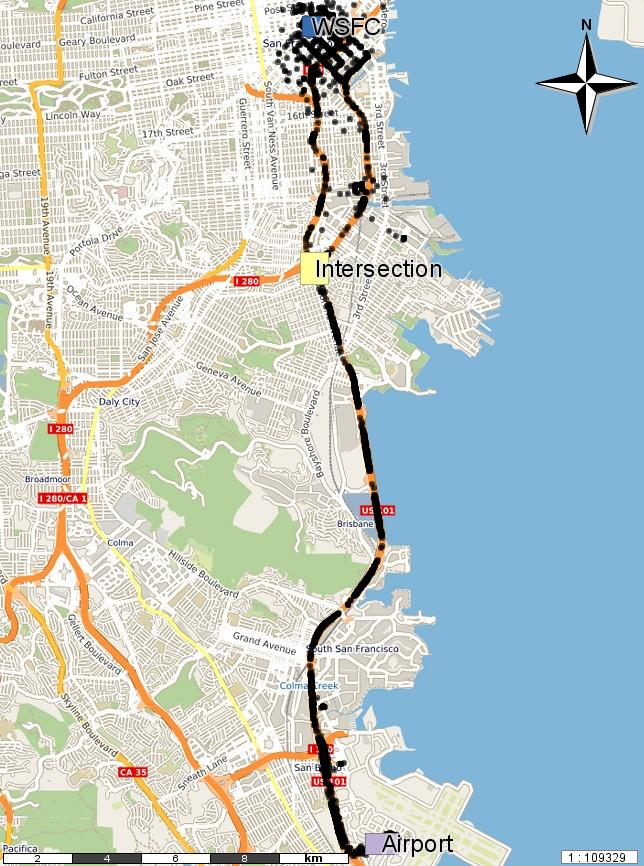
\includegraphics[width=.49\textwidth]{Images/CRAWDAD-Trajectories-Painted}
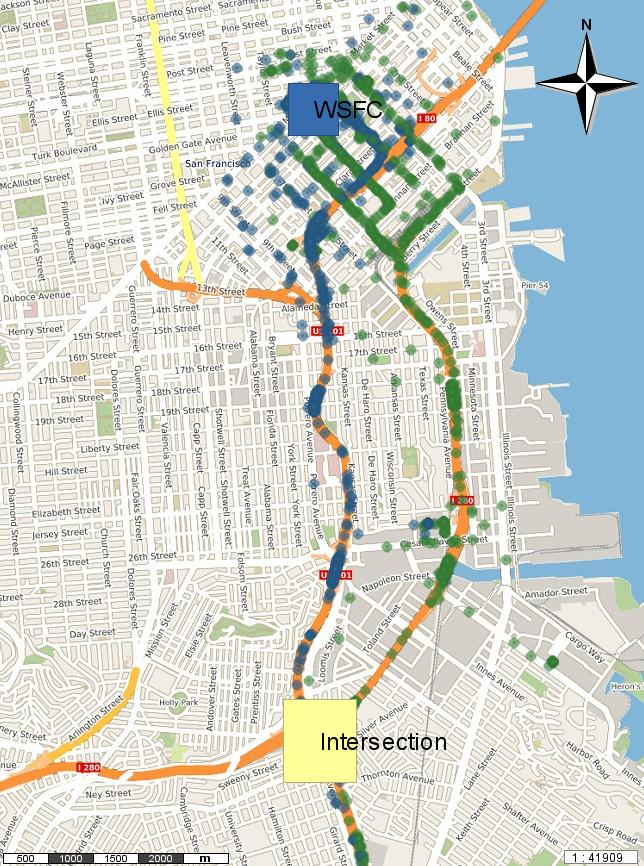
\includegraphics[width=.49\textwidth]{Images/CRAWDAD-Paths-Painted}
\caption{(left) CRAWDAD raw points (right) CRAWDAD Paths}
\label{fig:sanfrancisco_map_rois}
\end{figure}

With the objective of characterizing the trajectory movement, we separate the trajectories based on which road was used on the trip, whether 101 or 280, two major access roads to the city to WSFC. {Figure \ref{fig:sanfrancisco_map_rois}} (right) presents a zoom over trajectories moving on highways 101 (blue) and 280 (green) from Intersection to WSFC, where we can clearly visualize the different moves that connect both regions.

Considering the stops WSFC, Intersection, and Airport, we consider as the ground truth the four distinct paths followed by the trajectories that move between these regions. These paths are shown in Table \ref{tab:san_francisco_dataset}. All 25 trajectories moving from Airport in direction to WSFC via highway 101 are defined as class A1. The 101 trajectories moving in opposite direction from WSFC to the Airport by highway 101 belong to class A2. The 34 trajectories moving from Airport in direction to WSFC by highway 280 belong to class B1 and the 44 trajectories moving from WSFC in direction to Airport by highway 280 belong to class B2. We assume that trajectories that belong to the same class should be more similar than trajectories of different classes.

\begin{table}[h]
\scriptsize
  \centering
  \begin{tabular}{|c|c|c|c|c|}
  	\hline
 Direction & Highway & Trajectories & Class \\
  	\hline
 Airport to WSFC & 101 & 25 & A1\\
 WSFC to Airport & 101 & 101 & A2\\
 Airport to WSFC & 280 & 34 & B1\\
 WSFC to Airport & 280 & 44 & B2\\
    \hline
  \end{tabular}
  \caption{CRAWDAD dataset}
  \label{tab:san_francisco_dataset}
\end{table}

\subsubsection{Experimental evaluation}

In the following we describe the dimensions used to analyze the similarity of stops and moves. As spatial dimension of the stop we considered the centroid of the stop. As temporal dimension we used both start and end time of the stop, and as semantic information we used the name of the region (Airport, Intersection, and WSFC). For the moves, we use as spatial dimension the trajectory raw points of the move.

For measuring the similarity the following distance functions were considered for the stops.
\begin{itemize}
  \item Space: the Euclidean distance between the centroids of the stops:
	\item Time: let \textit{diam([t1, t2]) = $|t2 - t1|$} be the diameter of an interval; the time distance of two stops is given by the inverse of the proportion between the intersection of their intervals over the total period between the minimum starting time and the maximum ending time of their intervals, as given in equation \ref{eq:time_interval}
\begin{equation} \label{eq:time_interval}
	dist_t(a, b) = \dfrac{diam([a.t1, a.t2] \cap [b.t1, b.t2])}{diam([min(a.t1, b.t1), max(a.t2, b.t2)])}
\end{equation}
  \item Semantics: the distance is equal to 0 in case of exact match and equal to 1 otherwise
\end{itemize}

For the moves, we consider the following distance function:
\begin{itemize}
  \item Space: the spatial similarity of the moves is given by the UMS distance between the moves. We choose UMS because it is appropriate for low sampled trajectories, which is the case for this dataset, and it outperformed all existing similarity measures for raw trajectories evaluated in \cite{Furtado-UMS-2018}.
\end{itemize}

As several measures were not developed for semantic trajectories, for a more fair comparison we use existing measures over stops and over raw trajectories. For doing so we split the experiment in two parts: 1) a \textit{precision at recall} evaluation using only semantic trajectories; and 2) a \textit{precision at recall} evaluation using the raw trajectories. In (1) we run the experiment using the following measures: SMSM, MSM, DTWa, MSTP, CVTI, LCSS and EDR. In (2) we run the experiment for the following measures: MSM, DTWa, wDF, LCSS, EDR and UMS.

Table {\ref{tab:san_francisco_measures}} presents the dimensions used in each measure. To general multidimensional similarity measures as MSM, DTWa and MSTP, we provide as input all dimensions of each stop, namely: 1)  spatial information; 2) time interval; and 3) semantic information. We extend LCSS and EDR to support multiple dimensions, using the same strategy used in {\cite{Furtado:TGIS12156}}: given two multidimensional trajectories, two points are said as matched when all dimensions match, where each dimension has a distinct distance threshold. With those adaptations, both LCSS and EDR are used to measure similarity using the dimensions of space, time and semantics for stops. For CVTI, we provide as input the time interval of the stops and the stop names.

\begin{table}[!h]
\scriptsize
  \centering
  \begin{tabular}{|l|c|c|c|c|c|c|c|}
  	\hline
  & \multicolumn{4}{c|}{Semantic trajectories} & \multicolumn{2}{c|}{Raw trajectories} \\
 	\cline{2-5}
  & \multicolumn{3}{c|}{Stop} & \multicolumn{1}{c|}{Move} & \multicolumn{2}{c|}{} \\
 	\cline{2-7}
  & Space & Time & Semantic & Trajectory points & Space & Time\\
  	\hline
 SMSM & X & X & X & X & & \\
 MSM & X & X & X & & & \\
 DTWa & X & X & X & & X & X \\
 MSTP & X & X & X & & & \\
 CVTI & & X & X & & & \\
 wDF & & & & & X & \\
 UMS & & & & & X & \\
 LCSS & X & X & X & & X & X \\
 EDR & X & X & X & & X & X \\
    \hline
  \end{tabular}
  \caption{Dimensions used for each measure}
  \label{tab:san_francisco_measures}
\end{table}

Table \ref{tab:san_francisco_thresholds} shows the best thresholds used for measures that have thresholds. To define threshold values for the stops we experimented over a range of possible values of thresholds on each dimension (100m to 500m in a 100 meters step to stop spatial centroid distance and 0\% to 100\% in a 10 percentage points step to proportional stop time) and the best results obtained for each method were reported. For the move threshold the same approach was performed, varying the minimal distance for two moves match from 0 to 1 in a 0.1 unit step.

\begin{table}[!h]
\scriptsize
  \centering
  \begin{tabular}{|c|c|c|c|c|}
  	\hline
  & \multicolumn{3}{c|}{Semantic trajectories} & \multicolumn{1}{c|}{Raw trajectories} \\
 	\cline{2-5}
  & Space (meters) & Time proportion & Move & Space (meters) \\
  	\hline
 SMSM & 100 & 0.3 & 0.1 & - \\
 MSM & 100 & 0.3 & - & - \\
 MSTP & 100 & 0.8 & - & -  \\
 CVTI & 100 & 0.8 & - & -  \\
 LCSS & 100 & 0.3 & - & 100 \\
 EDR & 100 & 0.3 & - & 100 \\
    \hline
  \end{tabular}
  \caption{Thresholds used for each measure}
  \label{tab:san_francisco_thresholds}
\end{table}

\begin{figure*}[ht!]
\centering
\centerline{
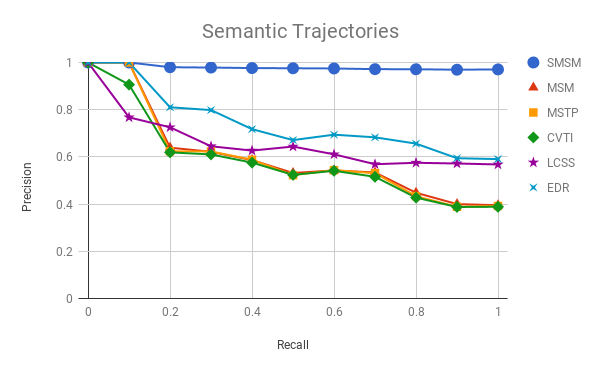
\includegraphics[width=0.5\textwidth]{Images/P_R-chart_San_Francisco.png}
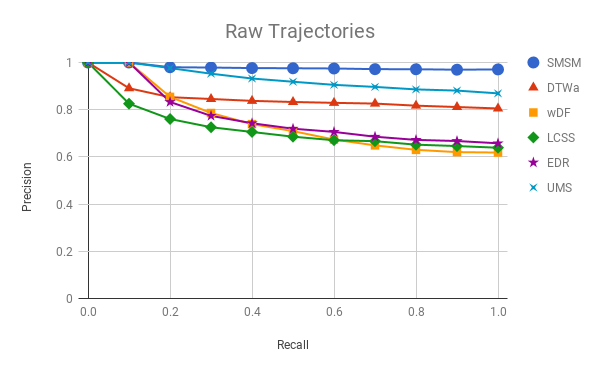
\includegraphics[width=0.5\textwidth]{Images/P_R-chart_San_Francisco-raw.png}
}
\caption{Precision at recall results for (left) semantic and (right) raw trajectories}
\label{fig:sanfrancisco_precision_recall}
\end{figure*}

\begin{table}[h]
\scriptsize
  \centering
  \begin{tabular}{|l|c|c|c|c|}
  	\hline
 & \multicolumn{2}{c}{Semantic} & \multicolumn{2}{|c|}{Raw} \\
 	\cline{2-5}
 & MAP & AUC & MAP & AUC \\
  	\hline
SMSM & 0.97 & 0.98& - & -\\
MSM & 0.57 & 0.60 & - & -\\
DTWa & 0.72 & 0.74 & 0.84 & 0.87\\
MSTP & 0.56 & 0.60 & - & -\\
CVTI & 0.55 & 0.58 & - & -\\
 wDF & - & - & 0.73 & 0.75\\
LCSS & 0.65 & 0.67 & 0.55 & 0.57\\
 EDR & 0.72 & 0.74 & 0.64 & 0.66\\
UMS & - & - & 0.92 & 0.93 \\
    \hline
  \end{tabular}
  \caption{MAP and AUC evaluation for CRAWDAD dataset}
  \label{tab:sanfrancisco_measures_map_auc}
\end{table}

Figure {\ref{fig:sanfrancisco_precision_recall}} presents the graphs with the results of the experiments on semantic and raw trajectories. As can be seen, SMSM out perform all other measures. Table {\ref{tab:sanfrancisco_measures_map_auc}} shows the MAP and AUC results for all measures, considering both semantic (Figure \ref{fig:sanfrancisco_precision_recall} left) and raw trajectories (Figure \ref{fig:sanfrancisco_precision_recall} right). The 1st and 2nd columns of Table {\ref{tab:sanfrancisco_measures_map_auc}} show that the results of SMSM(0.97/0.98) for MAP and AUC were significantly higher than MSM(0.57/0.60), DTWa(0.72/0.74), MSTP(0.56/0.60), CVTI(0.55/0.58), LCSS(0.65/0.67) and EDR(0.72/0.74) considering semantic trajectories. The 3rd and 4th columns in Table {\ref{tab:sanfrancisco_measures_map_auc}} show the comparison of SMSM with approaches developed for	 raw trajectories. The results show that SMSM(0.97/0.98) still outperform the other measures, being DTWa(0.84/0.87), LCSS(0.55/0.57), EDR(0.64/0.66), wDF(0.73/0.75) and UMS(0.92/0.93) less accurate. SMSMs best results in this experiment rely on its capability of handling both stops and moves together.

\subsection{Experiment with the Geolife Dataset}\label{sec:geolife}

The \textbf{Geolife} dataset is a well-known trajectory dataset, created by Microsoft Research Asia \cite{zheng2009mining} containing trajectories of 182 users, moving around Beijing, collected between April 2007 and August 2012. As a preprocessing step, we split trajectories when a 5 minutes gap between two consecutive points was found, since the trajectories of this dataset are highly sampled (lower than 2s).

\begin{figure}[ht!]
\centering
\centerline{
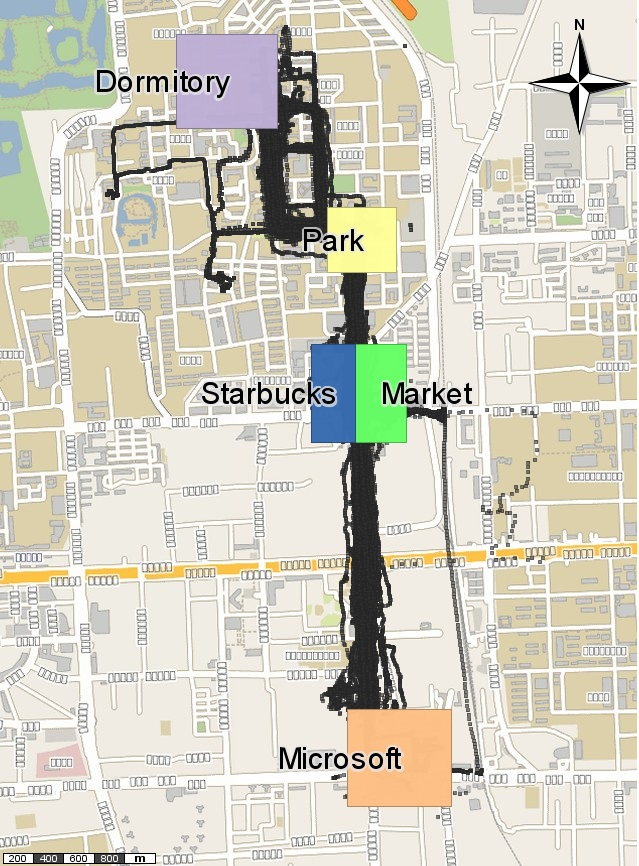
\includegraphics[width=.5\textwidth]{Images/Geolife-Trajectories-painted}
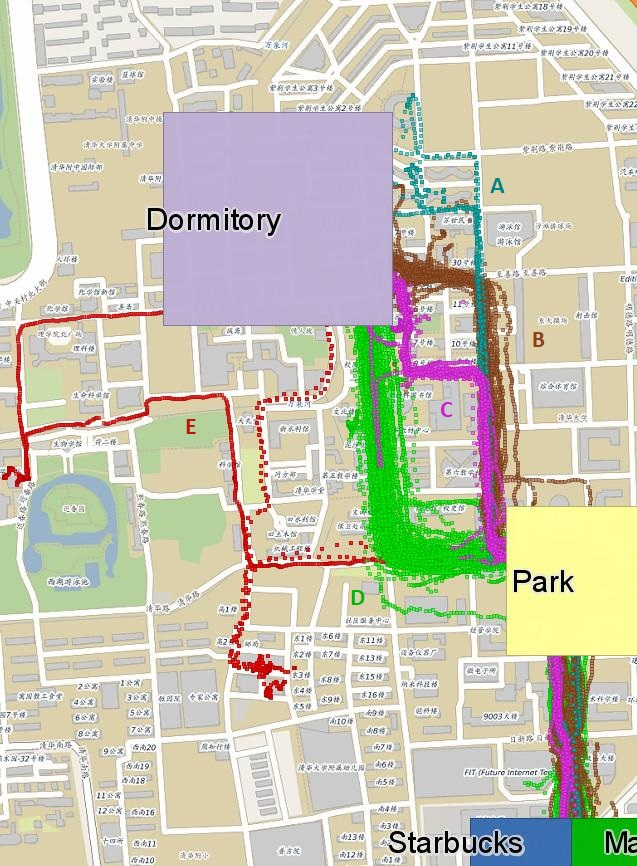
\includegraphics[width=.5\textwidth]{Images/Geolife-Paths-painted}
}
\caption{(left) trajectories moving between the regions Microsoft, Starbucks, Market, Park, and Dormitory (right) zoom over the distinct paths followed between Park and Dormitory}
\label{fig:geolife_map_rois}
\end{figure}

\subsubsection{Ground Truth Definition}
To build the ground truth, in this experiment we chose an area in Beijing, where pedestrians move between the University Dormitories and Microsoft Research Office. We considered five places as stops (Microsoft, Starbucks, Market, Park and Dormitory), that are show in Figure \ref{fig:geolife_map_rois} left. We considered 5 distinct paths connecting them, labeled as A, B, C, D, and E, as shown in Figure \ref{fig:geolife_map_rois} (right).

In Table \ref{tab:geolife_dataset} we define as ground truth 8 distinct classes of movement based on the sequence of stops and followed path: Microsoft to Dormitory via Market and Park by path A with 5 trajectories named as class A, Microsoft to Dormitory via Market and Park by path B with 40 trajectories named as class B, Dormitory to Microsoft via Park and Starbucks by path C with 11 trajectories named as class C, Dormitory to Microsoft via Park and Starbucks by path D with 115 trajectories named as class D1, Dormitory to Microsoft via Park and Market by path D with 7 trajectories named as class D2, Microsoft to Dormitory via Market and Park by path D with 149 trajectories named as class D3, Microsoft to Dormitory via Starbucks and Park by path D with 6 trajectories named as class D4 and Microsoft to Dormitory via Market and Park by path E with 4 trajectories named as class E.

\begin{table}[ht!]
\scriptsize
  \centering
  \begin{tabular}{|c|c|c|c|}
  	\hline
 Direction & Path &  Trajectories & Class \\
  	\hline
Microsoft to Dormitory via Market and Park& A & 5 & A \\
Microsoft to Dormitory via Market and Park& B & 40&B \\
Dormitory to Microsoft via Park and Starbucks& C & 11&C \\
Dormitory to Microsoft via Park and Starbucks& D & 115&D1 \\
Dormitory to Microsoft via Park and Market& D & 7&D2 \\
Microsoft to Dormitory via Market and Park& D & 149&D3 \\
Microsoft to Dormitory via Starbucks and Park& D & 6&D4 \\
Microsoft to Dormitory via Market and Park& E & 4& E \\
    \hline
  \end{tabular}
  \caption{Classes representing distinct paths for the ground truth}
  \label{tab:geolife_dataset}
\end{table}

\subsubsection{Experimental evaluation}

Using a similar methodology used for the first experiment, we calculate the precision at recall for all 8 classes in our ground truth, comparing the SMSM results to the other measures. The dimensions used for stops are: a) space; and b) the region name (Dormitory, Park, Starbucks, Market and Microsoft). For the moves we used the raw points of the move. The time dimension was not taken into account because in this experiment we have classes with few trajectories.

We consider the following distance functions for the stops.
\begin{itemize}
  \item Space: the Euclidean distance between the centroids of the stops;
  \item Semantics: the distance is equal to 0 in case of exact match and equal to 1 otherwise
\end{itemize}

For the moves, we consider the following distance function:
\begin{itemize}
  \item Space: the spatial similarity of the moves is calculated using the DTW distance between the moves. In this dataset we use DTW for the spatial distance because the trajectory points are highly sampled, and UMS is not a good measure when points are highly sampled as in the Geolife dataset.
\end{itemize}

Table \ref{tab:geolife_thresholds} presents the thresholds used in this experiment for each measure. As on the CRAWDAD experiment, we defined the thresholds by running each experiment over a range of possible threshold values and the best results for each method were reported. For raw trajectories, we evaluated as threshold values 2, 4, 6, 8 and 10 meters because this dataset is highly sampled and is of pedestrian trajectories. The threshold for the move dimension was defined as follows: two moves are said to match if the DTW distance between them is less than the sum of the Euclidean distance of the moves.

\begin{table}[!h]
\scriptsize
  \centering
  \begin{tabular}{|c|c|c|}
  	\hline
  & \multicolumn{1}{c|}{Semantic trajectories} & \multicolumn{1}{c|}{Raw trajectories} \\
 	\cline{2-3}
  & Space (meters) & Space (meters) \\
  	\hline
 SMSM & 100 & - \\
 MSM & 100 & - \\
 MSTP & 100 & -  \\
 CVTI & 100 & - \\
 LCSS & 100 & 4 \\
 EDR & 100 & 8 \\
    \hline
  \end{tabular}
  \caption{Thresholds used for each measure}
  \label{tab:geolife_thresholds}
\end{table}

Figure \ref{fig:geolife_precision_recall} (left) presents the precision at recall graph for this experiment. As can be observed, SMSM has the highest precision. Table \ref{tab:geolife_measures_map_auc} gives a better idea on the results. The 1st and 2nd columns of Table \ref{tab:geolife_measures_map_auc} show that SMSM results for MAP and AUC (0.93/0.94) were higher than MSM (0.70/0.72), DTWa (0.74/0.75), LCSS (0.74/0.75), EDR (0.74/0.75), MSTP (0.50/0.53), and CVTI (0.53/0.57). In addition, executing the experiment using raw trajectories (3rd and 4rd columns in Table \ref{tab:geolife_measures_map_auc}), the results of DTWa (0.86/0.87), LCSS (0.79/0.80), EDR (0.71/0.73), wDF (0.57/0.60), and UMS (0.84/0.85) did not reach the good results of SMSM.

\begin{figure*}[ht!]
\centerline{
\centering
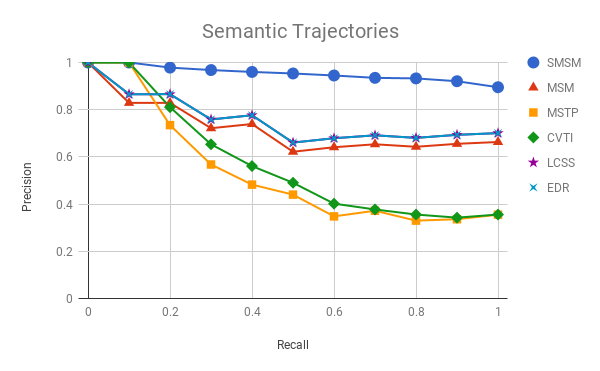
\includegraphics[width=.55\textwidth]{Images/P_R-chart_Geolife.png}
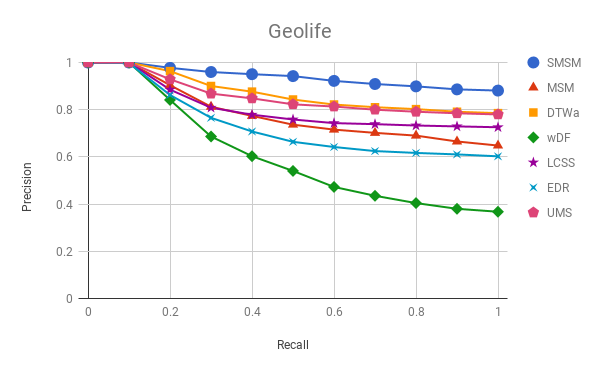
\includegraphics[width=.55\textwidth]{Images/P_R-chart_Geolife-raw.png}
}
\caption{Precision at recall results to semantic (left) and raw (right) trajectories}
\label{fig:geolife_precision_recall}
\end{figure*}

\begin{table}[ht!]
  \scriptsize
  \centering
  \begin{tabular}{|l|c|c|c|c|}
  	\hline
 & \multicolumn{2}{c}{Semantic}& \multicolumn{2}{|c|}{Raw}\\
 	\cline{2-5}
 & MAP & AUC& MAP & AUC\\
  	\hline
SMSM & 0.93 & 0.94 & - & -\\
 MSM & 0.70 & 0.72 & - & -\\
DTWa & 0.74 & 0.75 & 0.86 & 0.87\\
LCSS & 0.74 & 0.75 & 0.85 & 0.86\\
 EDR & 0.74 & 0.75 & 0.71 & 0.73\\
MSTP & 0.50 & 0.53 & - & -\\
CVTI & 0.53 & 0.57 & - & -\\
 wDF & - & - & 0.57 & 0.60\\
 UMS & - & - & 0.84 & 0.85\\
    \hline
  \end{tabular}
  \caption{MAP and AUC evaluation for the experiment with the Geolife dataset}
  \label{tab:geolife_measures_map_auc}
\end{table}

We notice that, in general, all similarity measures have a good result. However, we observed from the similarity scores that some measures having a high precision at recall, give a low similarity degree for trajectories of the same class that are highly similar. So to compare how well a measure can identify very similar trajectories of the same class, we perform another analysis: we extracted the mean similarity scores by class for each measure. We expect  all trajectories of the same class to be more similar between them, with higher similarity scores.
Table \ref{tab:geolife_similaritymeans} shows the mean similarity scores by class for each measure. For each measure, we choose the best AUC score, either from the semantic or raw trajectory results. The best results by class are in bold and the second better results are in italic. The results clearly show that the similarity score between trajectories of the same class is greater when using SMSM than all others measures. The other two better measures in this analysis can be said to be MSM and DTWa. LCSS, for instance, had a good result in precision at recall in Table \ref{tab:geolife_measures_map_auc}, but the average similarity show in Table \ref{tab:geolife_similaritymeans} was the second worst measure, showing that LCSS similarity is dominated by low matching scores.

\begin{table}[ht!]
\footnotesize
  \centering
  \begin{tabular}{|c|c|c|c|c|c|c|c|c|c|}
  	\hline
 Class & SMSM & MSM & DTWa & EDR & UMS & wDF & MSTP & LCSS & CVTI \\
  	\hline
 A & \textbf{0.87} & $0.61$ & \textit{0.62} & $ 0.59$ & $0.37$ & $0.20$& $0.26$ & $0.20$ & $0.15$  \\
 B & \textbf{0.69} & \textit{0.52} & $0.50$ & $ 0.41$ & $0.04$ & $0.05$& $0.03$ & $0.02$ & $0.01$ \\
 C & \textbf{0.88} & \textit{0.60} & $0.58$ & $ 0.46$ & $0.12$ & $0.11$& $0.09$ & $0.09$ & $0.05$ \\
D1 & \textbf{0.86} & $0.52$ & \textit{0.53} & $ 0.42$ & $0.08$ & $0.02$& $0.01$ & $0.01$ & $0.01$ \\
D2 & \textbf{0.76} & $0.59$ & \textit{0.60} & $ 0.55$ & $0.19$ & $0.14$& $0.14$ & $0.14$ & $0.06$ \\
D3 & \textbf{0.83} & \textit{0.51} & $0.51$ & $ 0.43$ & $0.08$ & $0.02$& $0.01$ & $0.01$ & $0.01$ \\
D4 & \textbf{0.78} & \textit{0.58} & $0.55$ & $ 0.53$ & $0.25$ & $0.22$& $0.20$ & $0.17$ & $0.12$ \\
E  & \textbf{1.00} & \textit{0.75} & $0.74$ & $ 0.71$ & $0.59$ & $0.38$& $0.45$ & $0.25$ & $0.25$ \\
    \hline
  \end{tabular}
  \caption{Mean similarities by class for each measure}
  \label{tab:geolife_similaritymeans}
\end{table}

In summary, what is shown in Table \ref{tab:geolife_similaritymeans} is that state-of-the-art measures give very low scores for multidimensional trajectories that follow very similar paths (same class).


\subsection{Experiment with sales promoter trajectories}
Another experiment was performed with a private company database compounded by the raw trajectories of sales promoters. A sale promoter is a brand's sales representative at retail stores, promoting products and assisting customers with brand's products. Usually, a sale promoter visit few stores in a day. This database contains the GPS raw trajectories of each sale promoter, from the start of his/her work day until the end of the work day.
In each store, the promoter spends some time (from 1 to 4 hours, usually) organizing brand's shelf, promoting products, replenishing stock, and so on. Much more time a promoter spends inside a store, more the brand is exposed to customer and more probably a customer will buy something. After that, the promoter moves to next store or end his/her workday. So, ideally, a promoter spends more time inside the stores than moving between the stores.

Each promoter trajectory was collected as follows: GPS coordinates are collected  every 10 seconds inside a 3 minutes interval of time, then the GPS collector sleep by 3 minutes, and then another interval of 3 minutes of points are collected.
To transform the raw trajectories in semantic trajectories, we run the CBSMoT as proposed by \cite{furtado:2017:cbsmot-like} and use the semantic trajectories as the sequence of \emph{stops} and \emph{moves} generated.

To evaluate our experiment, we use a ranking approach. We measure the quality of retrieved ranking by computing: i) Bpref - a metric that measures the number of times documents that are known to be non-relevant to an information need are retrieved before relevant documents \cite{BaezaYatesRibeiroNeto2011}; ii) NDCG - the Normalized Discounted Cumulative Gain, a ranking metric that measures the usefulness of a document based on its position in the rank\cite{BaezaYatesRibeiroNeto2011}; and iii) Spearman correlation coefficient - a correlation rank metric that compare two ranks and indicates both the direction and the alikeness of ranks, i.e., if both rank positions are increasing/decreasing in same or opposite direction and how much distinct it is the position of a same document in both ranks \cite{BaezaYatesRibeiroNeto2011}.

The Bpref metric indicates how non-relevant results affect the expected ideal rank. It is a good metric to evaluate the quality of retrieve techniques when not all data is known or its relevance is unknown. As said by \cite{BaezaYatesRibeiroNeto2011} ".., Bpref is a stable metric in the presence of incomplete information and can be used to compare distinct retrieval algorithms in the context of very large documents collections". On the other hand, NDCG is a rank metric that emphasizes relevant documents, measuring how much earlier that documents appears in the ranking. Spearman correlation coefficient "is likely the mostly used rank correlation metric" \cite{BaezaYatesRibeiroNeto2011}. It measures the correlation of two ranking by computing the differences between the positions of a same document in them.

\subsubsection{Ground Truth Definition}
To build up the ground truth dataset, in this experiment we chose promoters of one brand, resulting in 8939 raw trajectories of 122 distinct sale promoters.

\hl{Voce precisa explicar como gerou este ground thrut. quais criterios vc usou para gerar o ranking? Mostre uma tabela com as trajetorias de um promotor e o ranking e explique.}

\hl{quantas trajetorias tem o ranking de cada promotor? pode  ser a media}

\hl{Nao vi onde voce explica que usou o lcss para gerar o ground thruth. E se usaste o lcss para gerar o conjunto verdade, ele nao deveria acertar 100\%? Tinhas comentado que por ter usado o LCSS para gerar o conjunto verdade nao compararias com ele, mas agora comparas e ainda perdes do EDR.}

To construct all rankings we chose the best trajectory of each promoter and rank other trajectories from same promoter as how much similar they are for best trajectory. To define the best trajectory, we use a real metric from the private company: the best work day of any promoter is the day he/she spends, proportionally, more time inside a store then moving between stores.

\hl{Based on best trajectory of each promoter, we rank all other trajectories from same promoter, from the most similar trajectories (most close related sequence of \emph{stops}) to less similar.
The similarity between the best trajectory and all other trajectories of same user is given by the LCSS similarity between them. To compute the LCSS similarity is used only the spatial centroid of the \emph{stops}, using as spatial threshold 200 meters. On average, each ranking is composed by 72 }

\hl{Figure {\ref{fig:involves_best_trajectory}} presents the best trajectory of user $1289$ (left) and the four most similar trajectories of same user. The best trajectory has it first \emph{stop} at point A, pass through points B and C and goes to point D, going back to same store of point B. As Figure {\ref{fig:involves_best_trajectory}} shows, the two most similar trajectories have the same sequence of stops than best trajectory. On the other side, the third and fourth most similar trajectories have one \emph{stop} more and one \emph{stop} less than best trajectory, respectively.

Table {\ref{tab:involves_best_similarities}} shows the first four elements of similarity ranking of user 1289. As previously mentioned, the best trajectory (with Id 438) has two trajectories (with Id 325 and 558) with the same sequence of stores visited. The LCSS similarity of both is 1 where compared against the best trajectory. The third most similar (with Id 576) has one \emph{stop} more, leading to a LCSS similarity score of $0.8$. The fourth most similar trajectory (with Id 575) has one \emph{stop} less, resulting in a LCSS similarity score of $0.75$. In same way, all other trajectories of user are compared with best trajectory and it LCSS similarity score are computed.}


\begin{figure*}[ht!]
\centerline{
\centering
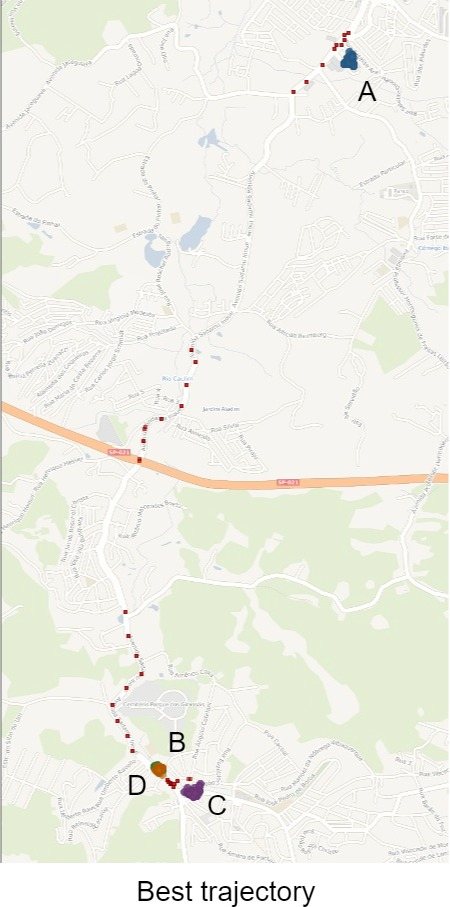
\includegraphics[width=.5\textwidth]{Images/Involves-BestTrajectory.jpg}
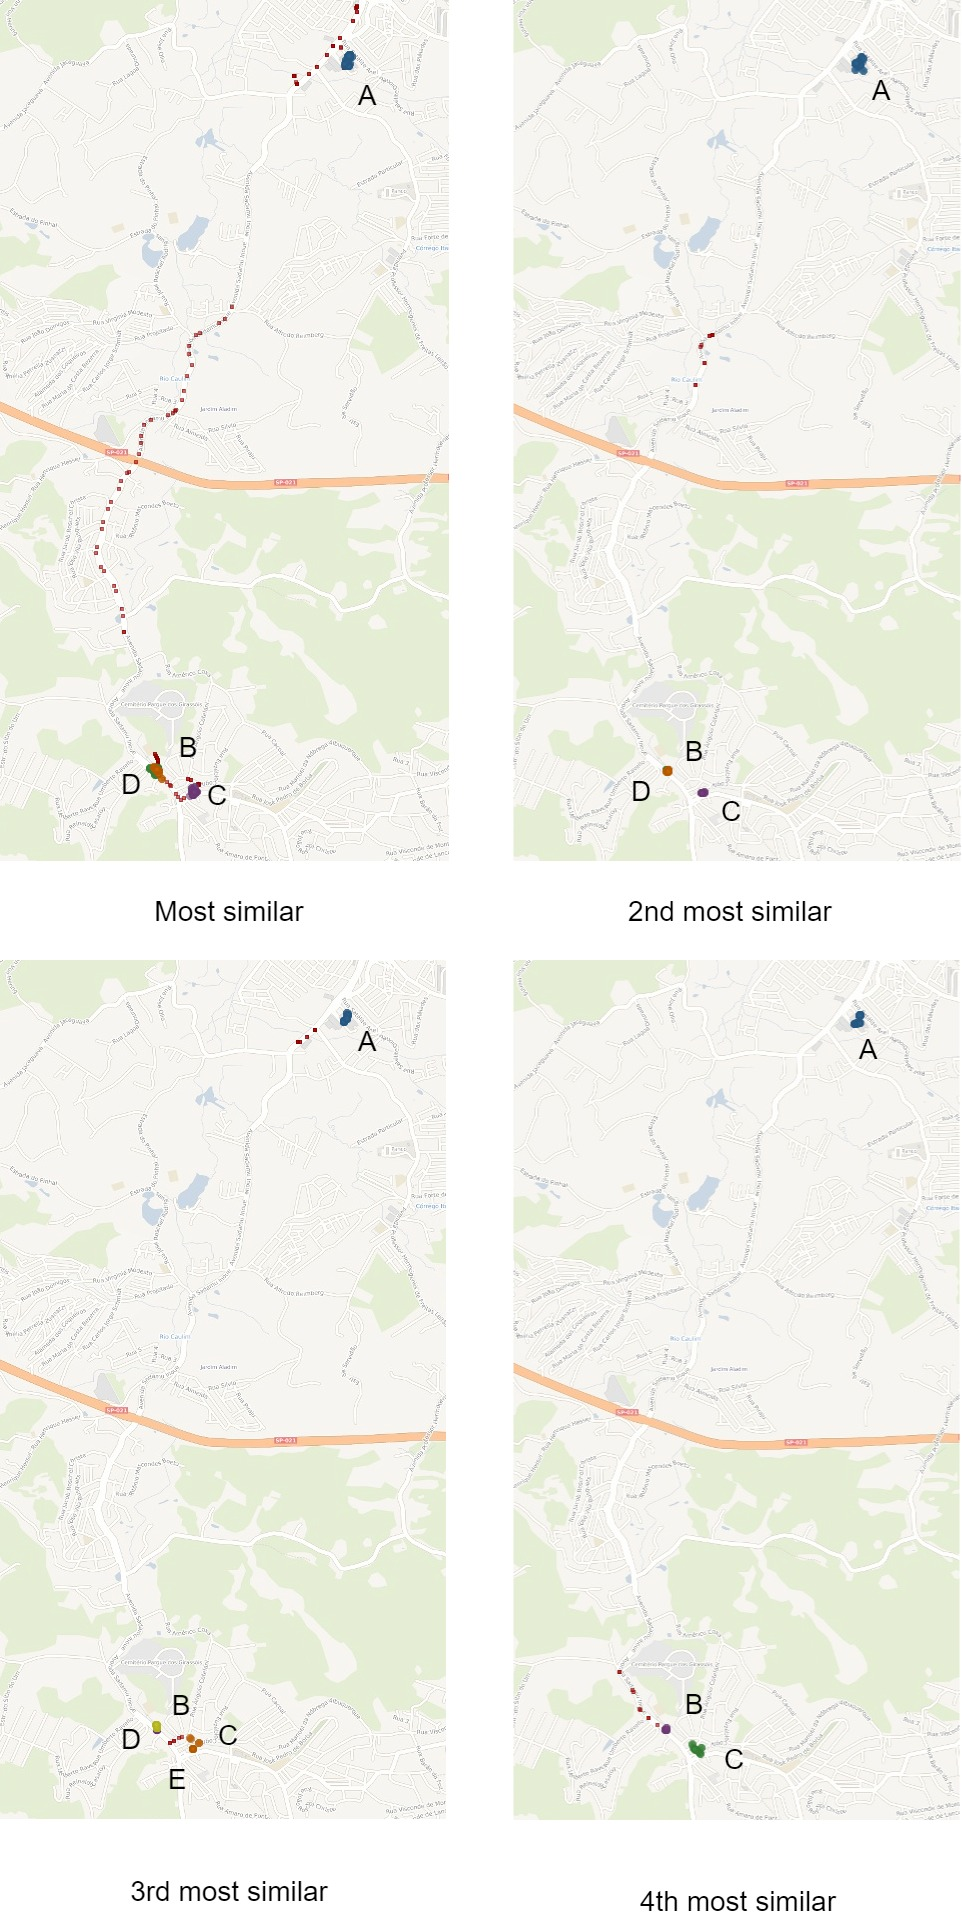
\includegraphics[width=.5\textwidth]{Images/Involves-MostSimilarTrajectories.jpg}
}
\caption{Best trajectory for user 1289 (left) and the 4 most similar trajectories of same user (right)}
\label{fig:involves_best_trajectory}
\end{figure*}

\begin{table}[!h]
\scriptsize
  \centering
  \begin{tabular}{|c|c|c|}
  	\hline
 Best trajectory Id & Most similar trajectory Id & LCSS spatial similarity \\
  	\hline
 438 & - & 1 \\
  & 325 & 1 \\
  & 558 & 1 \\
  & 576 & 0.8 \\
  & 575 & 0.75 \\
    \hline
  \end{tabular}
  \caption{LCSS spatial similarity of the best and the four most similar trajectories of user 1289}
  \label{tab:involves_best_similarities}
\end{table}


\subsubsection{Experimental evaluation}
In the following we describe the dimensions used to analyze the ranks generated by measures. As spatial dimension of the \emph{stop} we considered the median point occurred inside the \emph{stop}. As temporal dimension we used the total time duration that each \emph{stop} occurs. For the moves, we use the total time duration of movement between \emph{stops}.

For measuring the similarity the following distance functions were considered for the \emph{stops}.

\begin{itemize}
  \item Space: the Euclidean distance between the median points of the stops;
  \item Temporal: the distance is the proportion of the smaller time duration of one stop over the time duration of the other stop;
\end{itemize}

For the moves, we consider the following distance function.
\begin{itemize}
  \item Temporal: the distance is the proportion of the smaller time duration of one stop over the time duration of the other stop;
\end{itemize}

Unlike previous experiments, we performed this experiment using only semantic trajectories. We compare the generated ranks using the following measures: CVTI, DTWa, EDR, LCSS, MSTP, MSM and SMSM.

Table \ref{tab:involves_thresholds} presents the thresholds used in this experiment for each measure. As on all previous experiments, we defined the threshold by running the experiment over a range of possible threshold values and the best results for each measure were reported.

\begin{table}[!h]
\scriptsize
  \centering
  \begin{tabular}{|c|c|c|c|}
  	\hline
  & \multicolumn{2}{c|}{Stops} & \multicolumn{1}{c|}{Moves} \\
 	\cline{2-4}
  & Space (meters) & Time duration proportion & Time duration proportion \\
  	\hline
 SMSM & 200 & 0.5 & 0.5 \\
 MSM & 200 & 0.5 & 0.5 \\
 MSTP & 200 & 0.5 & 0.5 \\
 CVTI & 200 & 0.5 & 0.5 \\
 LCSS & 200 & 0.5 & 0.5 \\
 EDR & 200 & 0.5 & 0.5 \\
    \hline
  \end{tabular}
  \caption{Thresholds used for each measure}
  \label{tab:involves_thresholds}
\end{table}

Table \ref{tab:involves_measures_ranking} shows the results for each measure on each rank metric. SMSM had the better results in Bpref (0.59) and NDCG (0.82) and it had a tie with EDR in Spearman coefficient correlation (0.64). All other measures obtained worse results, as CVTI (0.13/0.39/0.39), DTWa (0.17/0.48/0.44), EDR (0.45/0.71/0.64), LCSS (0.22/0.58/0.51), MSM (0.51/0.81/0.52) and MSTP (0.16/0.45/0.39). The three ranking metrics chosen coverage some distinct kind of aspect in a ranking metric. 

\begin{table}[ht!]
\footnotesize
  \centering
  \begin{tabular}{|c|c|c|c|}
  	\hline
  & Bpref & NDCG & Spearman \\
  	\hline
CVTI & $0.13$ & $0.39$& $0.39$ \\
DTWa & $0.17$ & $0.48$& $0.44$ \\
EDR  & $0.45$ & $0.71$& \textbf{0.64} \\
LCSS & $0.22$ & $0.58$& $0.51$ \\
MSM  & $0.51$ & $0.81$& $0.52$ \\
MSTP & $0.16$ & $0.45$& $0.39$ \\
SMSM & \textbf{0.59} & \textbf{0.82}& \textbf{0.64}  \\
    \hline
  \end{tabular}
  \caption{Mean ranking measures for each measure}
  \label{tab:involves_measures_ranking}
\end{table}

\subsection{Scalability experiment}
The time complexity of SMSM is the same as LCSS, EDR, DTWa, CVTI, MSTP and MSM (\emph{O($n^2$)}). However, it is expected that SMSM performs worse than related approaches. It happens because as each \emph{movement element} is fully connected with neighbors \emph{movement elements} and share its \emph{stops}, each \emph{stop} will be computed twice, except the first and the last \emph{stop} of trajectory.

In order to evaluate the scalability, we perform the comparison of \emph{N} trajectories of Geolife dataset, which \emph{N} varies from 204 trajectories (the previously used dataset size) to 10,000 trajectories, by duplicating the existing trajectories until reach 10,000 trajectories. There are scenarios, such as in clustering techniques, where the pairwise similarity computation of all trajectories is required. As the main objective in this experiment is to compare the scalability of each measure exposed to hundred thousands or even millions of trajectory comparisons, the use of repeated trajectories is enough. \hl{O SMSM tambem eh mais lento porque executa sobre os moves o UMS, que eh a medida mais lenta para calcular similaridade em trajetorias brutas}

Figure \ref{fig:performance_comparison} shows the results in logarithm scale. In average, the execution times for SMSM were faster than DTWa and MSTP, 1.0-1.4x slower than CVTI,  EDR and LCSS, and 2.5x slower than MSM. However, it is important highlight that the results of SMSM are in same order of magnitude than the other measures and that its results showed greater precision in the retrieval-based experiments and rank-based experiment, with a relatively small increase in the computation time, thats show a trade-off with gains in precision with a little loss in performance.

\hl{Andre: faca um experimento de performance usando nos moves o UMS, dai certamente o SMSM ficara mais lento, mas faca um usando no move a distancia viajada ou velocidade media, que dai o SMSM deve ser mais rapido. Faca 2 versoes do SMSM no mesmo grafico}

\begin{figure*}[ht!]
\centerline{
\centering
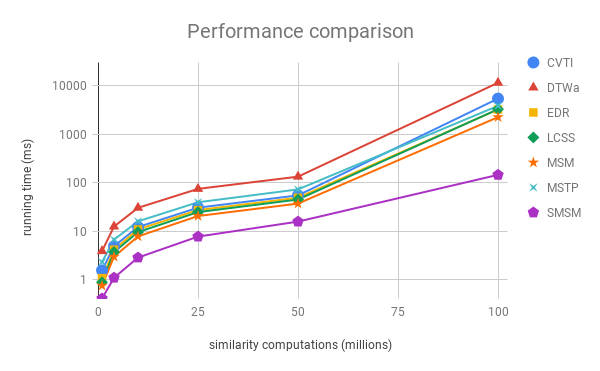
\includegraphics[width=\textwidth]{Images/Performance_comparison.png}
}
\caption{Scalability results: running time in milliseconds for a number of pairwise similarity computations}
\label{fig:performance_comparison}
\end{figure*}

\section{Conclusion} \label{sec:conclusions}
In this work we extended MSM to support both stops and moves and partial sequence matching. We call the proposed measure SMSM. To the best of our knowledge, SMSM is the first semantic trajectory similarity measure that deals with both stops and moves, and where both are heterogeneous elements. 
The proposed similarity measure is robust enough to consider multiple dimensions of stops and moves. A move, for instance, can be represented as raw points, the traveled distance, the major direction, the names of streets, etc.

We performed different experiments, using real data of distinct contexts, including taxi trajectories and pedestrian trajectories. By evaluating SMSM with an information retrieval approach, we show that SMSM was more accurate than other measures developed either for raw or semantic trajectories.

SMSM requires a full match between the start and end stop of two movement elements to evaluate the move. In future works we will study an extension of SMSM to evaluate the move in cases where the end stops of two movement elements do not have a full match.

\bibliographystyle{sbc}
\bibliography{sbc-template}

\end{document}
